\documentclass[12pt, a4paper]{article}
%%%%%%%%%%%%%%%%%%%%%%%%%%%%%%%%%%%%%%%%%%%%%%%%%%
\author{Patrick C. Shriwise}
\date{\today}
%\institute{Department of Engineering Physics, University of Wisconsin-Madison, 1500 Engineering Dr, Madison, WI 53706, shriwise\@wisc.edu}

%%%%% packages and defs
\usepackage{setspace}
\onehalfspacing
\usepackage{graphicx}
\usepackage{float}
\usepackage{amsmath}
\usepackage{booktabs}
%\usepackage{caption}
\usepackage{epsfig}
\graphicspath{{./images/}{../images/}{./}}
\usepackage[font={small,it}]{caption}
\usepackage{color}
\usepackage{hyperref}
\hypersetup{
    colorlinks=true, %set true if you want colored links
    linktoc=all,     %set to all if you want both sections and subsections linked
    linkcolor=black,  %choose some color if you want links to stand out
}

\makeatletter
\def\copyrightpage{
  \newpage
  \thispagestyle{empty}    % No page number
  \addtocounter{page}{-1}
  \section*{}            % Required for \vfill to work
  \begin{center}
   \vfill
   \copyright\ Copyright by \@author\ \the\year\\
   All Rights Reserved
   \newpage
\end{center}}

\begin{document}

\begin{center}
  \thispagestyle{empty}
  \addtocounter{page}{-1}
  \textbf{Improved Methods for Particle Tracking in CAD-Based Monte Carlo Radiation Transport} \\
  \bigskip
  by \\
  \bigskip
  Patrick C. Shriwise \\
  \bigskip
  A preliminary examination submitted in partial fulfillment of the requirements for the degree of \\
  \bigskip
  Doctor of Philosophy \\
  \bigskip
  (Nuclear Engineering and Engineering Physics) \\
  \bigskip 
  at the \\
  \bigskip
  UNIVERSITY OF WISCONSIN - MADISON \\
  \bigskip
  2016
\end{center}
\newpage
\copyrightpage

\tableofcontents 

\newpage
\section{Abstract}%%Status:Done%%

The performance of CAD-based Monte Carlo radiation transport relies heavily on its ability to return geometric queries quickly and robustly via ray tracing. The Direct Accelerated Monte Carlo (DAGMC) toolkit currently provides a robust ray tracing algorithm\cite{Smith_2011} given certain mesh requirements are met, but shortcomings of the underlying ray tracing kernel causes it to lag behind run times of a given Monte Carlo code using its native geometry engine. The current ray tracing kernel in DAGMC relies upon research in the areas of collision detection and rendering. Algorithms for collision detection involve moving geometry which isn't a concern in the area of radiation transport, and until recently rendering techniques have not aligned well with the needs of a Monte Carlo process. However, as new ray tracing kernels are developed for real-time, photo-realistic rendering, algorithmic approaches have appeared which are believed to be advantageous in radiation transport. In particular, the application of data parallelized ray tracing for Monte Carlo has been demonstrated - resulting in significant performance improvements. Single processor parallelization of this ray fire process cannot alleviate systematic performance problems coming from mesh features produced by the triangulation of CAD surfaces which are used to represent the model during transport. It is recommended that special attention be paid to these features when building acceleration datastructures to avoid performance degredation during particle interaction with those regions of the model. Algorithms for acceleration datastructures in rendering typically prioritize the time needed for the building of these structures, commonly leaving them less than optimal, but this results in an overall decreased time-to-render due to the balance of the build time with the the number of ray queries needed to generate the desired image or view. In radiation transport, the number of ray queries needed to generate the desired result is much larger than the number needed for rendering. As more time is spent ray tracing, the build times of the underlying acceleration structures becomes less significant, thus the balance between time spent building these structures and the time using them for ray tracing must be reconsidered in this context. It is hypothesized that in the case of large and geometrically complex problems for which DAGMC is intended, extra time spent optimizing the ray tracing acceleration datastructures via adaptation to troublesome mesh features may result in reduced overall runtimes. Finally, a preconditioning scheme is presented to avoid unecessary ray queries when particles are far from cell boundaries based on implicit surface techniques used in rendering. It is hoped that the combined effect of these improvements will allow DAGMC to provide CAD-based Monte Carlo simulations with performance on the order of the native codes it supports, thus alleviating the concern for additional computational time while maintaining the benefit of reduced human time and effort in model preparation.

\section{Introduction}%%Status:Done%%

%% The purpose of this document is to outline the current state of the art in spatial partioning hierarchies for the purpose of improving performance in DagMC. It will take into account as much of the existing literature as possible. An analysis of the literature will also be conatined, identifying areas for improvement within the context of ray tracing for the specific application of Monte Carlo ray tracing.

Monte Carlo methods are a class of algorithms employed to solve complicated physical systems or mathematically complex problems which are difficult or impossible to solve analytically. As such, these methods are well suited for solving 3D neutron transport problems representing real-world systems. In the Monte Carlo process, the path and energy of particles are tracked from their birth until their termination through a series of simulated collision events which are collectively defined as a particle's history. If a particle is scattered during one of these events, its direction and energy changes and it moves on to the next collision or event. If the particle is absorbed or escapes the system, the particle's history is terminated. Throughout this process, the material or volume in which the particle exists will determine physical quantities which influence the randomly-selected events the particle encounters. It is therefore necessary to know when the particle is moving from one volume to the next through out its lifetime. In the organization of most Monte Carlo codes, an event arises in the particle's history and the distance to this event along the particle's direction from its current position is determined. It is then important to know whether the location of the particle's next event lies inside or outside of the volume in which the particle currently exists. If the event location lies inside the volume, then the particle can step forward to that location and the event will be recorded as part of that particle's history. If the event location lies outside of the volume, the event cannot be considered valid as it could be taking place inside of a new material with different physical properties with respect to the particle which in turn changes the physics governing the particle's transport. In this situation, the particle is then moved forward along its current direction vector to the surface of the current volume and is logically moved to the volume on the other side of that surface. At this point the particle's history continues and its next event will be selected via the Monte Carlo process.

In order to determine if the event location lies inside the current volume, the closest distance to the boundary of the volume along the particle's current trajectory must be found. The most common queries of interest in many Monte Carlo codes being a point containment query to determine which volume the particle lies in and the closest surface intersection to a particle's location along its current trajectory. The tracking of particles through the virtual space of a model occupies is a problem commonly encountered in the area of computational modeling. There are many approaches to this problem, each having its own advantages and disadvantages.

Most Monte Carlo geometries come in the form of Constructive Solid Geometry (CSG). CSG allows one to form a complex volume from a set of Boolean operations on CSG primitive objects such as cylinders, spheres, parallelepipeds, etc. CSG allows for an exact representation of these objects via their analytical forms. This in turn allows for the direct calculation of the nearest surface intersection for a given particle location and direction, also defined as a ray, by performing ray intersection checks for each of the CSG objects which make up the volume and using the smallest of these values. Given that these checks can be done using the CSG surfaces' analytical forms, the necessary geometric queries required for Monte Carlo can be returned quickly to the physics code throughout the particle's history in $O(S)$ time, where $S$ is the number of surface objects used to define the volume.

In practice, there are limitations associated with the use of CSG as a geometry representation. First, there is a practical limit to the complexity of volumes that can be formed using CSG objects. CSG volume formations require human knowledge and verification of the primitive object combinations required to form each volume in the model. Given that in most current implementations these models are formed via a text-based implementation, highly complex volumes can be extremely difficult to create and modify. As a result, a large amount of human time is spent generating and verifying modules of complex real-world systems. In reality, there are volumes which are impractical to represent due to the difficulty of their representation using these methods. These objects are typically modified in Monte Carlo models to be an approximation of the intended object, each approximation or feature removal requiring its own justification for its effect on the outcome of the desired solution. The consequence of this in the broader scope of engineering analysis is that a different model is then used for structural, thermal hydraulic, magnetic, and other domains than for radiation transport. Many of these other areas already take advantage of CAD systems for their geometric representation, allowing for accurate representation of the real world systems and faster design iteration. Based on well-established methods such as finite element analysis etc. on CAD-based models, this provides significant motivation for radiation transport on CAD models as well.

The use of CAD models allows for radiation transport on arbitrarily complex or highly detailed models - allowing one to almost exactly represent the intended model as closely as current modeling methods allow. Though as the geometric representation becomes more intricate, particle tracking during transport becomes increasingly difficult. Ray-intersections with analytical forms of CAD surfaces and volumes are sometimes impractical or impossible to compute over entirety of the object's domain. To circumvent this problem, the surfaces are triangulated by the CAD graphics engine to provide a generalized representation for each surface in the form of a triangle mesh via the Direct Accelerated Geometry Monte Carlo (DAGMC) toolkit \cite{Tautges_2009}. These triangle meshes are generated such that all points on the mesh are within a specified tolerance of the analytical representation of the surfaces, meaning that all features of the model on larger than this tolerance are present during transport. While the number of geometric objects increases by $O(10^5)$, all geometric queries from the Monte Carlo code can then be handled the same way despite the volume's form or complexity. Robustness can also be a challenge when using CAD-based models, often times caused by poorly defined mesh entities at surface interfaces. It has been shown, however, that transport on CAD models can be performaed with equivalent reliability as that of a CSG based system \cite{Smith_2011}.

Currently, the performance of CAD-based transport is slow in comparison to its CSG counterpart. As will be discussed later in this work, CAD-based transport can be many times slower, causing delays of hours, days or weeks depending on the parameters of the problem at hand. In part, this is caused by the necessary triangulation of surfaces. On one hand, the problem of finding the closest or next primitive object of intersection is now more difficult due to the large number of triangle primitives needed to represent complex models. However, the problem has now been generalized to the search for a nearest ray-intersection with a common geometric primitive in the volume, a well researched-problem known as ray tracing. Ray tracing is most commonly used to generate 2D images by simulating photon ray-interactions with virtual 3D objects in a process known as rendering. These light rays are typically cast from the perspective of the view to be generated, and pixel colors are determined by the reflections, refractions, etc. of the photons on their course from the view origin to the light source. To a certain degree this process is a naturally analagous to Monte Carlo analysis despite the differing physical regime of the particle's transport underlying the final image. For highly detailed models containing millions of triangles, a linear search of the primitives for the next intersection is out of the question in terms of computational expense. As a result, extensive research has been done in the area of acceleration data structures for ray tracing which partition the problem space in order to establish a binary search over the geometric primitives of the model to accelerate the nearest intersection search. Using acceleration datastructures oriented toward these spatial searches, geometric queries can be satisfied in $~O(log(T))$ time, where T is the number of triangles needed to define the volume.


%In realistic renderings, it is sometimes possible that light rays may scatter before reaching the next virtual object on their path. In order to determine if this will occur before reaching the next object, the distance to interaction (scattering or otherwise) must be compared to the distance to the next object just as in the Monte Carlo process for radiation transport.

The acceleration datastructures currently used in DAGMC were adapted from work on object interference detection in 1996 \cite{Gottschalk_1996} as an adapted form of datastructures commonly used in rendering. This particular datastructure is a binary tree hierarchy of oriented box bounding volumes used to rapidly reduce the number of primitives in the geometry query to a small set which are then tested for geometry query of interest. This datastructure was chosen for the relatively shallow hierarchy it produces so that it may work well within a mesh database framework which is not necessarily oriented toward binary search performance. Recent work in the area of ray tracing in conjunction with the re-emergence of common chipset architectures oriented toward single instruction multiple data (SIMD) implementations has increased the performance of CPU based ray tracing kernels significantly \cite{Wald_2008}, allowing a proof of concept for CAD-based radiation transport which competitive with the performance of CSG based implementations.

This document will discuss the background and theory of several different areas surrounding particle tracking and ray-tracing in CAD-based Monte Carlo, the current state of ray tracing acceleration datastructures, and other optimization techniques of interest in Chapter \ref{background}. Chapter \ref{experiments_and_data} will go over some previous work investigating sources of performanc limitations in current CAD-Based transport. This will begin with an evaluation of a CAD-based geometry library developed at the University of Wisconsin-Madison, DAGMC, in comparison to the native CSG kernel it replaces. Next, a particularly problematic feature seen in CAD-based meshes will be examined. Then a proof of concept for CAD-based Monte Carlo competitive with that of native codes will be presented. Finally, a set of further improvements for ray tracing kernels applied to robust particle tracking in CAD geometries will be proposed in Chapter \ref{research_proposal}. 


\section{Background}%%Status: In Progress%%
\label{background}


\subsection{Acceleration Datastructures for Ray Tracing}
\label{subsec:accel_datastructures}

Acceleration datastructures for ray tracing are designed to rapidly narrow the search for a location in virtual space given a starting position and orientation. This is accomplished by sectioning the space using various partitioning constructs in either the spatial or entity dimensions. These paritions are determined by a division heuristic which establishes the datastructure topology and partition for a set of geometric primitives. After partitioning, the primitives are then associated (either implicitly or explicitly) with the partitions that contain them. This processes recurs until conditions for leaf creation are met which can be based on a maximum number of associated primitives, the space the partition occupies, or some other heuristic. The most effective heuristic for ray tracing to date is the Surface Area Heuristic (SAH). This heuristic provides a way to select the best of a set of candidate split planes and also determine if current partition has met leaf conditions of the hierarchy. The SAH uses the surface area of candidate child partitions relative to the current partitions's surface area as an approximation for the probability that the child will be visited after the parent volume. The explicit form of the surface area heuristic was introduced in 1987 by Goldsmith and Solmon \cite{Goldsmith_1987} and later formalized by MacDonald and Booth in 1990 \cite{MacDonald_1990}. Its full form is found in Equation \ref{eq:SAH}.


\begin{figure}[H]
  \begin{equation}
    C =  C_{t} + \frac{SA(B_{L})}{SA(B)} |P_{L}|C_{i} +  \frac{SA(B_{R})}{SA(B)} |P_{R}|C_{i}
    \label{eq:SAH}
  \end{equation}
  \begin{align*}
    C_{t} - & \,cost\, of\, traversal\, to\, child\, nodes \\
    C_{i} - & \, cost\, of\, primitive\, intersection\, check\, \\
    SA() - & \, gives\, surface\, area\, of\, bounding\, volume \\
    B_{L} - &  \, bounding\, volume\, of\, left\, child \\
    P_{L} - & \, primitives\, contained\, by\, the\, left\, child  \\
    B_{R} - & \, bounding\, volume\, of\, right\, child \\
    P_{R} - & \, primitives\, contained\, by\, the\, right\, child \\
    B - & \, parent\, bounding\, volume \\
  \end{align*}
  \caption{Full form of the surface area heuristic.}
  \label{fig:SAH}
\end{figure}

The cost of each split done in the tree is evaluated as the cost of an extra traversal downward in the tree, as well as the cost of the intersection checks for each primitive contained by the child nodes as if they are leaf nodes. Both of the children will not always be intersected by a ray however so the cost is then adjusted by some estimation of the probability that a ray which visits the current partition will also intersect the child of that partition. In the surface area heuristic this probability is estimated as the surface area of the child partition divided by the surface area of the parent partition. The cost of the primitive intersections are conatined by the child partition are then weighted as such. In reality, a better estimation of child node intersection probability would be given by the relative cross section of the child/parent partitions with respect to the ray direction. Given that ray directions are unknown a priori, the surface area serves well enough for applications with uniform ray distribution. This heuristic is used to produce the highest quality datastructure achievable by today's standards and is generally regarded as the best method in many production ray tracers to date. It is also highly adaptable to many types of acceleration datastructures in ray tracing, including the types discussed below.

\subsubsection{KD-Trees}%%Status:Done%%

The KD-Tree or multidimensional binary search tree was originally developed as a method for querying records in databases and has since found use in other applications including speech recognition, global information systems, and ray tracing \cite{Bentley_1975}.  KD-Trees operate by recursively dividing the dimensions of the problem in a spatial manner with each dimension being split in a different level of the tree. The resulting subsets of this split are linked to the node as children of the current node and the process continues until leaf conditions are met. Entities are listed as contained by a partition only if they are contained by all parents of the partition as well, meaning that all entities lie within a node's partition for each dimension of the problem.

This process is easily applied to the virtual 3D space of CAD models for ray intersection queries. The problem space is divided evenly in the x dimension. The two child partitions are then divided along the y axis and the resulting children of this division are subdivided along the z axis. Divisions are typically done in such a way that the space of the current candidate is bisected, however it is possible that by doing this primitive entities are divided by the plane as well. There are a couple of ways in whicih this problem is handled. The first is to simply reference any intersected primitives in both of the subdivisions. This has the effect of creating a small overlap between the partitions and means that some primitives may be checked for intersection more than once, but requires no changes to the original model. The other solution is to divide the primitive entities using the parition plane.  This solution requires alterations to the model which may be undesirable under certain conditions and violates the description of the KD-Tree as a pure querying structure by making modifications to the existing model.

%% 2-D Example from Bentley1975 here %%
\begin{figure}[H]

  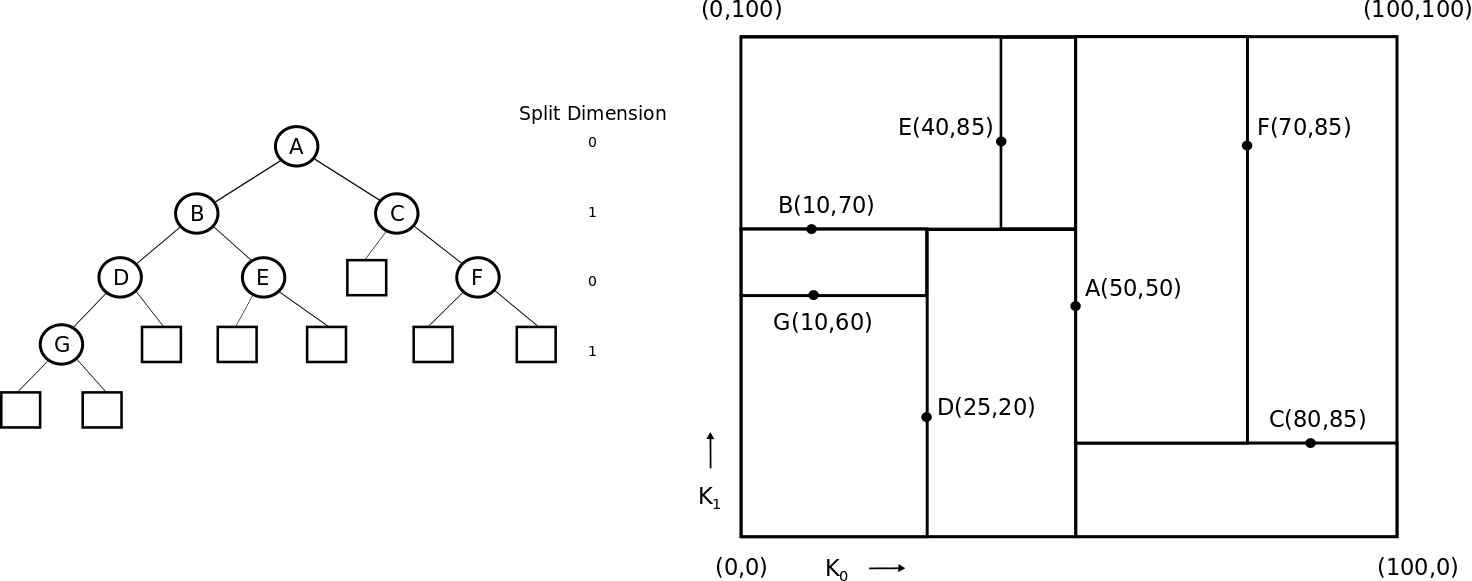
\includegraphics[scale=0.25]{2d_kd_eg.png}
  \caption{Two dimensional KD-Tree example adapted from Bently et. al. \cite{Bentley_1975}. Left: Graph representation of the KD-Tree. HISON's are right children. LOSON's are left childre. Boxes are null. Right: Two dimensional space partitioned in the graph. Boxes represent the range of their respective subtree.}
  \label{2dkd}
\end{figure}

KD-Trees are able to out-perform many other acceleration datastructures due to traversal schemes developed based on the inherent quality of KD-Trees' non-overlapping sibling nodes. As a KD-Tree is being constructed, an ever-shrinking bounding box is being defined as one moves deeper into the tree. At the leaves of a KD-Tree a well-resolved bounding box can be conceptualized using the coordinates of the last six splitting planes visited. The conceptual construction of this box is one way to move from node to node in a more efficient way than a more standard depth-first approach used in tree traversal. The partitions whose planes are used to construct this conceptual box can be linked to the current partition in order maintain a spatially localized search within the hierarchy. These links are referred to as neighbor links and, as shown by Samet et. al.\cite{Samet_1989}, can be used to significantly reduce traversal costs in the KD-Tree. During traversal if a leaf is visited its neighbor links can be used to direct the query to either the next adjacent leaf or a nearby interior node in the tree thus avoiding a depth-first style traversal in which the next step upon visiting a leaf node is to return to the root node of the tree and continue. These neighbor links take advantage of the idea that if a leaf node is visited, but the desired intersection is not found, then it is likely that the desired intersection is close to the current leaf location. In this way, one can avoid large amounts of unecessary shallow and middle level tree traversal steps.

\subsubsection{Bounding Volume Hierarchies}%%Status: Done%%

KD-Trees are frequently citied as being able to provide the best ray tracing performance to date \cite{Ernst_2007,Hurley_2002,Havran_2000}. In particular, KD-Trees are noted as being better equipped to handle models with highly varying triangle sizes/densities. In practice, bounding volume hierarcies are more commonly used, however, for their lower memory footprints and well-developed parallel building schemes. These features are of great import for systems with limited memory, such as GPUs, and applications with intent for realtime viewing or interaction. These requirements do not necessarily apply to the realm of Monte Carlo particle tracking which is commonly performed on CPUs which have more memory available relative to GPUs.

The initial concept of using the bounding volume construct as a pre-check for ray-intersection with CSG objects was introduced by Weghorst in 1984 \cite{Weghorst_1984}. Weghorst explored the possibility of using bounding spheres and bounding boxes to contain geometric objects. This work also went so far as to create a hierarchy the object-based bounding volumes, noting the importance of hierarchicaly joining bounding volumes near to each other in space so as not to have parent volumes containing large amounts of empty space between the bounding volumes being joined.

\begin{figure}[H]
  \centering
  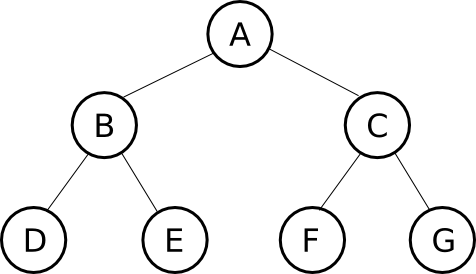
\includegraphics[scale=0.3]{binary_graph.png}
  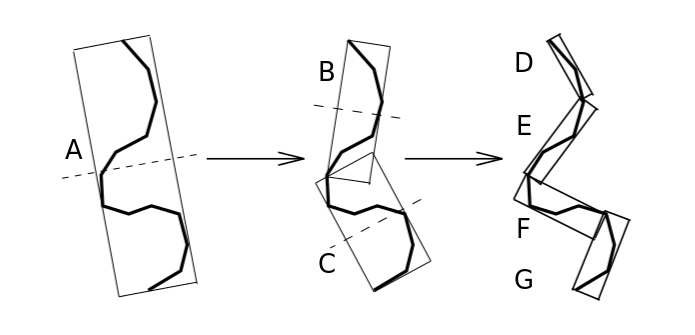
\includegraphics[scale=0.3, trim = 0 50 0 0 ]{bvh_2d_ex.png}
  \caption{Two dimensional BVH example adapted from Gottschalk 1996 \cite{Gottschalk_1996}}
  \label{2dbvh}
\end{figure}

%% As CAD systems improved, it was found that complex geometric objects become difficult to render as the analytic calculation of ray intersections became more costly. As a result, representations of geometric objects were then triangulated for rendering purposes. Ray interactions with these more simple triangle primitives are much less costly to compute in comparison to the previous analytic representation. Given that the geometric object can be discretized accurately, this also allows for the rendering of arbitrarily complex geometric objects without the need for continuous development of efficient analytic intersection techniques for all classes of complex parametric surfaces. 

In Weghorst's exploration of sphere and box bounding volumes it was found that while spherical bounding volumes are less compuationally expensive to check for ray intersections than bounding boxes, the latter generally provide a tighter fit to the objects they contain. This tighter fitting is important as it decreases the chance of wasted ray-volume intersection checks for rays which intersect the bounding volume but not the object it contains. When considering the application of bounding volumes to a discretized analytic surface represented by a triangle mesh, this becomes even more important as BVHs become deeper when constructed on large numbers of primitive entities and more ray-volume intersection checks are performed to reach leaf nodes. Even applied to analytical objects, this effect was reflected in the results of Weghorts's work strongly enough to show that bounding boxes provided better performance in accelerating the ray intersection process than bounding spheres.

Two forms of BVHs are commonly applied in ray tracing problems: Axis-Aligned Bounding Boxes (AABBs) and Oriented Bounding Boxes (OBBs). AABBs are boxes whose orientation is restricted such that their faces are parallel to the global planes of the problem space. In practice, tightly fitting axis aligned boxes are straightforward to construct given a set of points to contain, and overlaps between the children of a parent box are minimal. Their simple representation results in a relatively low memory footprint and straighforward, robust ray-intersetion tests. Unlike AABBs, the faces of oriented bounding boxes are allowed take any orientation relative to the global axes in order to enclose their set of primitives as tightly as possible. Several robust methods for determining the orientation of a box for best fit to a set of primitives have been discovered \cite{Gottschalk_1996,ORourke_1985}. OBBs are better for avoiding superfluous ray-box intersections that might otherwise occur for an axis aligned box and more quickly conform to the full set of enclosed primitives as the boxes are recursively divided. By orienting their axes with the local set of pimitives they are bounding, candidate splitting planes, usually based on the current box axes, are more effective at separating primitive entities and reaching leaf conditions more quickly. This leads to more shallow hierarchies making the worst case number of intersection tests lower than for an axis aligned box hierachy on average. While a shallow hierarchy might indicate a smaller memory footprint, OBBs require one to store some extra information about their orientation relative to the global axes making this assumption difficult to consistently prove. One disadvantage of oriented boxes encounterd upon hierarchy traversal is that the intersection check requires an extra step in transformation of the ray to the oriented axes of the box in question. The information needed for this basis transformation of the ray must be constructed and applied to the ray before the box intersection can continue as it would for an axis aligned box. So while the oriented box hierarchy may have fewer intersection checks to do for a given ray query than an axis aligned box, the intersection checks are inherently more expensive than in the case of AABBs. In practice, AABBs are commonly used in BVH's for their simplicity of implementation and well-researched ray intersection algorithms. Other reasons for this preference will be discussed later in Section \ref{subsec:arch}.

There are multiple approaches to constructing such datastructures given a set of geometric primitives, but only top-down approaches will be discussed here. A top down approach begins with a single bounding volume enclosing all primitives. At this point, child boxes of this root volume are created by selecting a splitting plane for the box which divides the primitves contained by the current bounding volume into two subsets. This process is then repeated until leaf conditions are met. The selection of candidate splitting planes and the selection of a final plane for splitting based on its estimated worth can greatly affect the performance of the datastructure. A virtually infinite set of planes could be tested to find the optimal plane for dividing the entities between the two child volumes, but even if one were to encounter such a splitting plane, it can be difficult to identify the plane as such without more knowledge about the final tree structure. As a result, a limited set of planes is tested for the best split based on a set of assumptions about the problem at hand and some heuristics shown to provide the best performance. The most common method for split plane candidates is median plane splitting in which a bounding volume is split in half for each axes of the current bounding volume. The splitting planes are then evaulated and the best plane is selected based on some estimation of its performance based on some heuristic. The most effective heuristic to date being the surface area heuristic described at the beginning of this chapter.

One difficulty that bounding volume hierarchies of any type face is that of overlapping sibling bounding volumes. Overlapping sibling volumes can cause additional box intersection checks in a similar manner to loosely fitting bounding volumes. If a ray enters a region of overlapping sibling volumes, this causes the children of both boxes to be checked despite the fact that the ray will eventually only intersect with the desendants of one box or the other. Overlaps are difficult to avoid, however, due to the reality that volumes are required to contain discrete elements for robustness, not just a section of the virtual space. Simply put, if the splitting plane of a bounding volume goes through one of the geometric primities, there will be an overlap in the resulting child volumes. As one can imagine, this is more often the case than not. This inefficiency can be exacerbated by the structure of triangulated objects the BVHs are being formed around. The overlaps found in AABBs are typically limited to the size of perhaps one or two geometric primitives. Fortunately, there are ways to cope with this problem.

The spatial BVH variant (SBVH) was introduced by Stich et. al. in 2009 \cite{Stich_2009} with an additional complexity to the node splitting step. As candidate split planes are considered, the duplication of triangles (or geometric primitives) to be contained in both resulting nodes. This grants much more freedom when considering how a node should be partitioned. Conversely, this extra freedom expands the search space of an optimal split plane for the node, making the process more complex. The relatively simple application of this method is performed by considering both splits in which triangle duplication is prohibited and splits in which it is allowed. In the sceanrio for which triangle duplication is prohibited, the set of candidate planes is equivalent to that of a standard BVH building algorithm. Stich applies the surface area heuristic for the purpose of his publication. In the case for which reference duplication is allowed, the search for a splitting plane is much more open - as previously mentioned. In fact, the search becomes fundamentally aligned with the search for a spatial split as might be found in a KD-Tree implementation. The optimal splitting plane is then selected via a comparision of the SAH cost for all candidate split planes - spatial or traditional. Secondary heuristics are used to limit reference splitting in an effort properly manage the datastructure's memory footprint. The result of the SBVH is a hierarchy which can be traversed just like any other BVH but with significantly reduced sibling volume overlaps. The general effect of the allowance for reference splitting during construction is more tightly fitting bounding volumes and reduced sibling volume overlap. Their results consistently show significant improvement over other methods, ranging anywhere from (20-100\%).\cite{Stich_2009}

%% The BVH is currently the most commonly employed acceleration datastructure for ray tracing due to its reduced memory footprint in comparison to the other datastructures discussed in this chapter. They are relatively simple to implement for the performance they are able to provide and have a smaller footprint relative to most other ray tracing acceleration datastructures.

\subsubsection{Octrees}%%Status:Done%%
\label{sec:octree}
Octrees are a partitioning scheme in which cuboid bounding boxes known, also known as voxels, are used to partition the problem space into the 8 quadrants defined by the axes and extents of the parent voxel. These 8 voxels are then identified as children of the parent voxel. This process is repeated recursively until leaf conditions are met for the voxel. This typically means that the voxel contains a set number of primitive references and the branch should be ended. This spatial subdivision technique is commonly used to efficiently index data in 3-D space.\cite{Glassner_1989} Octrees exist somewhere in the space between KD-trees and BVHs in that their divisions are spatial, partitions contain no overlaps, and placement of entities in nodes occurs in a similar manner to that of KD-trees, but each node is represented by a well-defined bounding volume as in a BVH.

Octrees can consume a large amount of memory relative to the other data structures previously discussed in this chapter. It is often possible that voxels may be completely devoid of underlying entities. There are typically many voxels containing no primitive references but may be required to exist as part of the datastructure. This results in many voxels being stored in memory which aren't useful other than to verify that the space they contain is empty. Additionally, geometric primitives may be referenced multiple times if they intersect multiple nodes thus increasing the required memory storage with the same consequence as seen in KD-Tree traversl with the possibility of a primitive being checked more than once upon traversal. The memory footprint is mostly of concern in applications for visualization on GPUs which have applied new methods for representing octrees.

\begin{figure}[H]
  \centering
  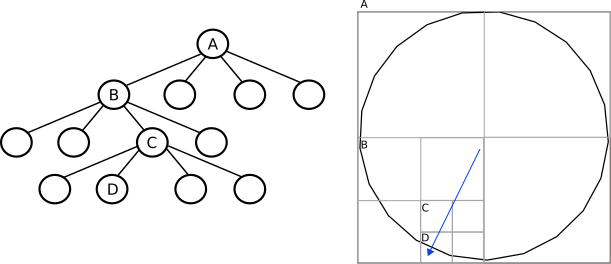
\includegraphics[scale=0.65]{octree_2d_ex.png}
  \caption{Two dimensional Octree example of a top-down ray fire traversal for a simple geometric object.}
  \label{octree_2d_ex}
\end{figure}

One advantage of octrees is the cubic nature of the partitioning voxels. The value of a node in hierarchies such as these (or in the BVH for that matter) lies in its ability to remove candidate space from the query, yet a voxel can only accomplish this if rays strike the voxel. The result is that one measure of a voxel's value can be described by the ratio of its probability of an intersection check to the space it will exclude from the query search or its volume. In a problem with a uniform ray distribution, the probablity of a ray to intersect a given voxel can be related to a voxel's surface area. Thus cubic voxels have the most favorable ratio possible based on their geometry. The uniformity of voxel properties provide a predictable nature of the octree which is advantageous when traversing the data structure as well. 

The predictable size and location of any given node in the tree determined from the root node properties also provides a fast lookup of the deepest node in the tree containing a point in space. This is helpful in providing a starting point for ray traversal which is not the root node, allowing one to avoid shallow traversal steps. Additionally, octrees have non-overlapping nodes which allows for efficient traversal schemes similar to the neighbor linked traversal done in KD-trees. These traversals are conceptually similar to that of the KD-tree's but typically employ some form of Morton encoding to determine which node in the octree the ray should visit next \cite{Revelles_2000}. Other traversal techniques allow the octree to avoid creating and traversing nodes containing empty space which can significantly reduce its memory footprint in cases where internal nodes of the tree aren't required to define some spatial dataset as mentioned above \cite{Samet_1989}. These methods are often applied in GPU environments due to the limited memory available there. Octrees are often used to store spatial data fields as well, providing higher resolution of the field near boundaries of the field's domain as the voxels become smaller in that region. As mentioned above, octrees are known for having prohibitively large memory footprints than other datastructures, but they can also be used advantageously for a combined purpose if a problem requires the storage of one or more well-resolved data fields near volume boundaries as well as the capability for some form of ray tracing.


\subsection{Architecture Based Acceleration}%%Status: Pending%%
\label{subsec:arch}

This section will focus on the advantages of vectorization implementations or Single Instruction Multiple Data (SIMD) oriented programming. When considering the problem of parallelism in computing, programmers focus on one of two areas: \textit{functional parallelism} or \textit{data parallelism}. Functional parallelism describes the method of performing multiple operations in parallel on many processors while data parllelism describes operation on multiple datasets at the same time on a single processor. SIMD is a form of data parllelism in which, as the name indicates, the same set of numerical operations are performed on multiple sets of data in parallel. Chipsets with support for SIMD instructions became very popular in the mid-1990s as the home PC became more common and demand for multimedia-related performance increased. In response, many CPU manufacturers at the time such as Intel, IBM, and Motorola began to release products with SIMD instruction sets. The most powerful of which was Intel's Streaming SIMD Extensions (SSE). Over time, CPU clock speed became the larger focus of many manufacturers due to dramatic gains in processor speed. As processor speed increases began to wane or push the limit of current cooling technology in the early 2000's, a new shift toward mult-core designs occured. Currently, as CPU clock speeds remain somewhat steady in multi-core systems, a focus on single-thread performance via SIMD has returned to great effect. Newer SIMD instruction sets such as Intel's Advanced Vector Extensions (AVX or AVX2) have been able to provide double the width of operable data, allowing for a theoretical doubling of performance in SIMD enabled codes \cite{Hughes_2015}.

SIMD execution has found use in many different areas including medical imaging, financial analytics, database management, computer visualization, and physical simulation. As is the case in any problem well-suited to parallel programming, all of these applications perform the same set of computations many times on large sets of data. This kind of situation arises quite often in applications related to modeling or visualizing the real world. One common indicator of a problem which would benefit from parallel programming is the presence of a few common sets of operations done many times or in a recursive manner. Looking at the problem of ray-tracing, the traversal of any of the partitioning data structures discussed in Chapter \ref{subsec:accel_datastructures} relies heavily on a couple of key operations: hierarchy ray-node intersections and ray-primitive intersections. The ability to do intersection checks of many nodes at once or many triangles at once has obvious benefit when satisfying geometric queries during simulation or rendering. Several demonstrations of ray-tracing data structures adapted to take advantage of SIMD-enabled optimizations on modern CPUs have already been developed.

\begin{figure}
  \centering
  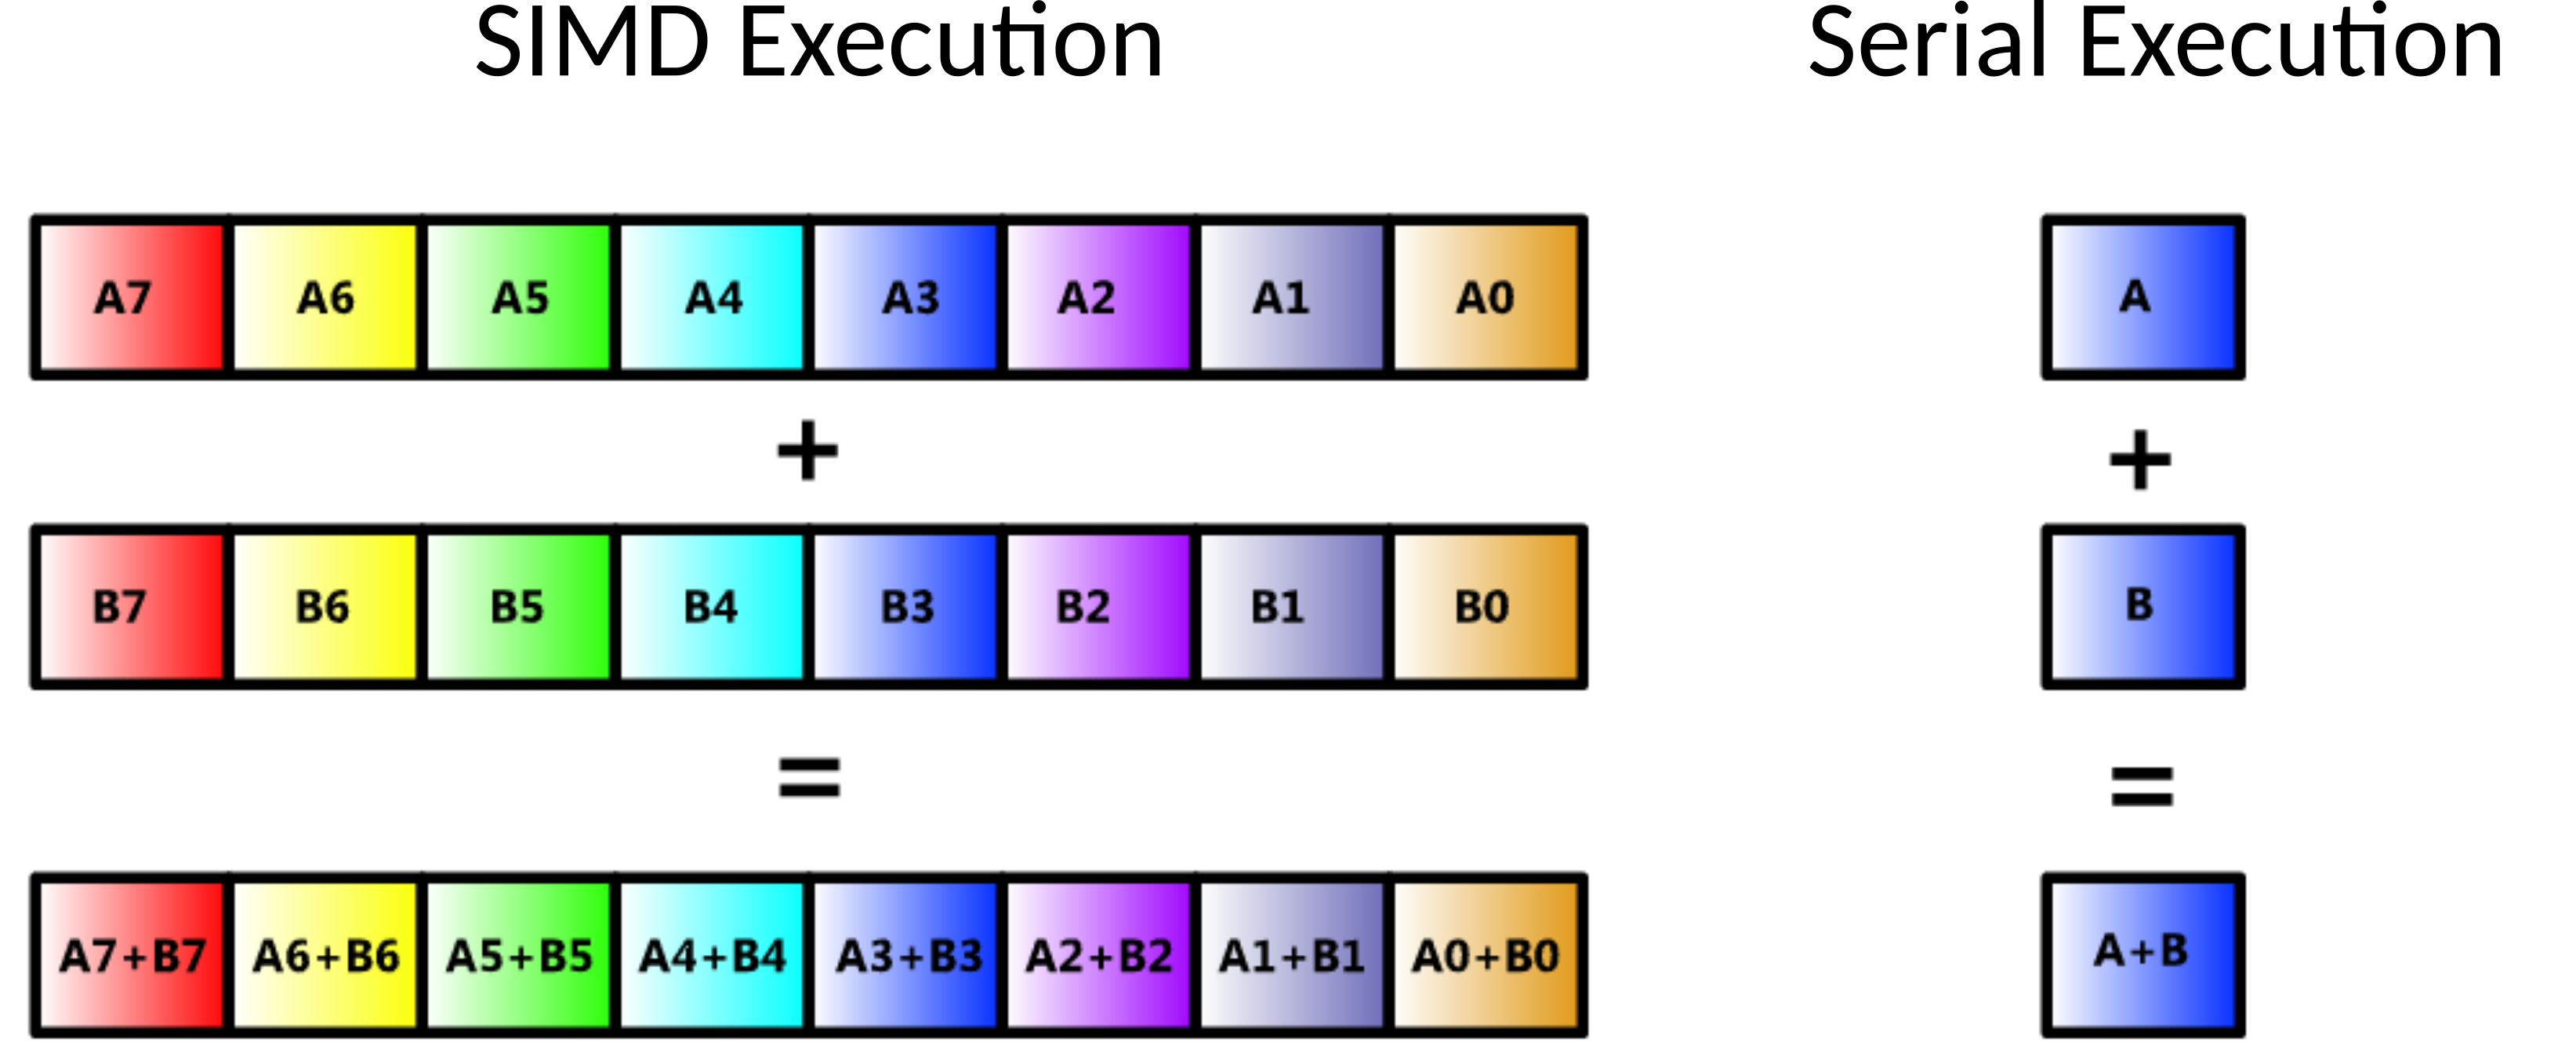
\includegraphics[scale=0.6]{simd_ex.png}
  \caption{Concept of data parallelism using SIMD. Adapted from Intel's documentation on the advanced vector extensions instruction set. \cite{Intel_AVX}}
  \label{simd_ex}
\end{figure}

An early implementation of SIMD used to intersect a ray with many triangles at the leaf nodes of a KD-Tree was performed by Hurley in 2002 \cite{Hurley_2002}. This implementation demonstrated a signifiant improvement in ray-primitive intersection performance and established many significant observations about the utilization of SIMD commands within ray tracing applications. Despite the fact that the cost of primitive intersection checks was reduced, most of the time spent satisfying the ray query was spent in traversal of the hierarchy to the leaf nodes. Noting that the number of triangles in the KD-Tree's leaf nodes were small in comparison to the SIMD registry width, Hurley described two ways in which to further exploit data parallelism of SIMD in ray tracing. One method is to traverse and intersect multiple rays at the same time. This is refereed to as the N:1 approach. The other is to intersect more triangles with a single ray which is referred to as the 1:N approach. A key component of the former method is that the group of rays being intersected have very similar traversal paths through the hierarchy so they may be grouped together in a packet for a narrow traversal path. This property is known as ray coherence. Branching off of Hurley's work, Wald demostrated that rays can be effectively grouped into packets and traversed in a binary space partitioning tree (a modified KD-Tree) to achieve performance equal to that the high-end graphics hardware of the time \cite{Wald_2001}. As more realistic physical effects are being applied to ray tracing kernels such as light-scattering surfaces or fog, rays paths become less coherent, meaning that the same or very similar primary rays will not necessarily follow similar paths through the model or its underlying acceleration hierarchies. Due to this problem-dependent lack of ray coherency, the latter method of data parallelism in which a single ray is intersected with many hierarchy elements in a single step was revisited. Wald wisely observed that taking advantage of SIMD operations in traversal of a KD-Tree is difficult due to its binary nature. He goes on to state that the KD-Tree's superior serial performance in comparison to that of serial BVH implementations drove reluctance to move away from the KD-Tree and resulted in the establishment of ray packets. \cite{Wald_2008} Both Wald and Dammertz \cite{Dammertz_2008}, concurrently presented implementations of SIMD enabled traversal and primitive intersection on multi-branching BVH's in 2008. Both implementations showed impressive performance enhancements, ranging anywhere from 3-10 times faster than the baseline ray tracing kernels used for comparison.

Both Wald and Dammertz approached the construction of multi-branching BVH's in the same way. Each built a standard binary BVH using the adjusted SAH cost analysis in Figure \ref{adjusted_SAH} with median plane splitting. They then collapsed the tree by directing child nodes to their ancestors to achieve the desired branching ratio. Wald opted to use a more exotic, graphics-oriented, architecture  with Intel's Larrabee and was able to apply a branching ratio of 16 to his BVH while Dammertz used a branching ratio of 4 using Intel's Streaming SIMD Extensions (SSE). While a higher branching ratio provides higher SIMD utilization, Wald recognized that for common implementations branching ratios between 4 and 8 would be optimal for most common architectures.

Axis aligned bounding boxes were used in both Wald and Dammertz's implementations. While oriented bounding boxes have been shown to conform more quickly to the underlying geometry and can generate more shallow trees than axis aligned bounding boxes, axis aligned bounding boxes are more favorable for a couple of reasons. First, oriented bounding boxes require more information to be stored about their orientation relative to the global problem axes. This extra information can limit how many nodes will fit into a single SIMD step and it is often more beneficial to check more axis aligned boxes at once than fewer oriented bounding boxes at once when traversing the hierarchy. This is partially because more nodes can be fit into the SIMD register to be visited at once, and partially because axis aligned boxes have faster ray intersection tests without the re-orientation of the ray information to the box coordinates. Secondly, though oriented bounding box hierarchies are more shallow than their axis aligned counterparts', the bounding volume hierarchies in these implementations are made more shallow manually through a higher n-ary structure of the tree. 

\begin{figure}[H]
  \begin{equation}
    C = C_t + \sum_{k=0}^{K} \frac{SA(B_k)}{SA(B)}\frac{|P_k|}{T}C_i
  \end{equation}
  \begin{align*}
    K - & \, number \, of \, desired \, children \, per \, interior \, node \\
    T - & \, number \, of \, triangles \, in \, SIMD \, register
  \end{align*}
  \caption{An adjusted form of the surface area heuristic as presented by Wald in \cite{Wald_2008}. Note: some notation has been modified to agree with notation used earlier in this work.}
  \label{adjusted_SAH}
\end{figure}

For completeness of the ray tracing datastructures discussed in Chapter \ref{background}, SIMD implementations of Octree's were sought out, but none were found. This is likely due to the fact that SIMD registers on common architectures are not yet wide enough to accomodate 8 nodes are not yet common. It is also worth noting that while the KD-Tree is restricted to a binary hierarchy, another variation, the bounding interval hierarchy, might be compatible with SIMD traversal of interior nodes \cite{Watcher_2006}. 

%%Not sure if this justification really belongs here, but I can move it later.%
These shallow BVH structures optimized using SIMD instruction sets could be of great use in the area of radiation transport. Other than primary rays from specific source types, ray queries coming from underlying physics codes in Monte Carlo transport are largely incoherent. Particles are much more likely to interact in certain media than others and these event locations as well as post-event directions are selected by a physically biased random selection process whereas most traditional rendering kernels encounter more predictable interactions at the boundaries between objects in the model, enabling them to take advantage of ray packet tracing as discussed above. It is interesting to note that as ray tracing kernels attempt to create more realistic environments, they experience a decrease in coherency large enough for the field to consider other means such as single-ray SIMD traversal to maintain improved performance. In fact, several works exist describing quasi Monte Carlo methods being applied in rendering, as noted by Dammertz \cite{Dammertz_2008}. Additionally, shallow BVH structures naturally have a smaller memory footprint. This property is also desirable in the world of Monte Carlo radiation transport as the CAD-based models which this work focuses on become increasingly more complex in the number of triangles. As SIMD registers gain width in time both performance enhancements and reduced memory footprints of datastructures will become more pronounced.

%% SIMD is a form of complex instruction set computing (CISC) which combines operations that are often done together to make them more efficient. More specifically, SIMD provides the capability to apply the same operation, or set of operations, to independent data elements. Because this is done in a single processor thread, it is classified as data parallelism. 

\subsection{Implicit Surface Representations}%%Status: Done%%
\label{implicit_surfaces}

An implicit surface is a multivariate function defined over an $ R^3 $ domain as:

\begin{equation}
    \Omega(R^3)\rightarrow R
\end{equation}


Implicit surfaces are rich and versitile representation of closed manifolds used for modeling, simulation, and rendering. Additionally, implicit surfaces can be used to generate triangle meshes for rasterization or rendering on GPUs \cite{Sethian_1996} and can also be constructed from arbitrary triangle meshes or point clouds \cite{Sigg_2006}. Implicit surfaces are defined using the isocontour of a scalar function defined over all space unlike an \textit{explicit} representation of a surface which defines the subset of space which the boundary occupies. Intuitively it might seem wasteful for a definition to be true for all space considering the relatively small amount of space the object will occupy, however a number of powerful tools for geometric modeling using these representations will be discussed in this section.

An isocontour of this function with the value, $v$, can be described as:

\begin{equation}
  \Omega(\vec{x}) - v  = 0 
\end{equation}

For simplicity, the boundary of an implicit surface is defined as the isocontour for which $v=0$. As a result, inside of the surface will have a negative value while any point outside of the surface will have a positive value.

Unlike their explicit counterparts, implicit representations allow complex topologies of surfaces to be integrated into a single representation. This is in part because the function is defined for all space.As a result they handle the merging and separation of disparate volumes well. These properties allow for straightforward representation of dynamics surfaces such as fluids though this is not of concern in the area of radiation transport. In practice, implicit surfaces are used to extract mesh representations of surfaces, re-sample the model into some other proxy for the geometry, and render models via ray tracing. Implicit surfaces are well-suited to these applications due to the integrated geometric properties that can be quickly recovered from their analytic forms. 

Important geometric information needed for vizualization and simulation can be readily recovered from implicit surface representations. For example, a common operation in particle transport is the determination its containment by a volume in the model. A quick evaluation of the implicit function for this point will indicate its containment by the sign of the function. Such a process is more complex in the case of an explicit or discretized representation. Typically this involves casting a ray through the model and counting up the intersections or relying on the orientation of triangle normals to indicate an entering or exiting intersection. The oddness or eveness of the number of crossings will then determine the points containment. Additonally, the distance to nearest intersection with the surface from any point in space can quickly be determined via the definition of a signed distance function, $d(\vec{x})$, formally defined as:

\begin{align}
  & d(\vec{x}) = min(|\vec{x} - \vec{x_{I}}|) \\
  & \Omega(\vec(x))  \,s.t.  \,|\Omega(\vec{x})| = d(\vec(x)) 
\end{align}
\begin{equation*}
  d \, - \, signed \, distance \, function
  \vec{x_{I}} \,- \,nearest \, boundary \,intersection
\end{equation*}

Meaning that implicit surface functions meet these three requirements of a signed distance function:

\begin{figure}[H]
  \begin{itemize}
  \item $ \Omega(\vec{x}) = d(\vec{x}) = 0 $ for all $x$ on the surface boundary
  \item $ \Omega(\vec{x}) = -d(\vec{x}) $ for all $x$ inside the surface boundary
  \item $ \Omega(\vec{x}) = d(\vec{x}) $ for all $x$ outside the surface boundary
  \end{itemize}
\end{figure}

As a result, the nearest distance to the implicit surface for any point can be found by evaulating its signed distance function, $|\Omega(\vec(x))|$. This enables very quick distance queries regarding the proximity of a point to the nearest point on the surface for rendering processes such as ray casting. Nearest intersections along the direction of the ray can also be found directly by solving the analytical form of the implicit surface for a ray with origin, $\vec{c}$ and direction vector, $\vec{v}$, using  $\vec{x} = \vec{c} + t\vec{v}$ and solving for $t$, but robust methods for this process do not exist for higher-order surfaces. An alternative method given a ray origin and direction, is to find the minimum distance from the ray origin to the surface with a signed distance function. The ray can then be clipped by this distance along is direction vector. This process will repeat until the nearest distance to the surface has eventually reached a near-zero value at which point the intersection of the ray with the surface has been found. The distance of the ray's origin to the intersection can be returned as the distance from the current location to the original ray location.

In comparison to other visualization approaches, implicit surfaces and their derived signed distance functions have a very small memory footprint due to their analytical nature, and as mentioned previously geometric information critical to visualization processes can be determined with ease. To define even more complex models, implicit surfaces can be easilty represented as a boolean combination of surfaces. The union or intersection of two surfaces can easily be defined using:

\begin{align*}
  Intersection: & \, min(\Omega_{A}, \Omega_{B}) \\
  Union: & \, max(\Omega_{A}, \Omega_{B}) \\
  Difference (A-B): & \, min(\Omega_{A}, -\Omega_{B}) \\
\end{align*}

Surface representations commonly found in CSG are a simple subset of implicit surfaces. However, limiting oneself to a set of pre-defined surfaces requires the boolenan combination of many surfaces to define highly complex objects which can be accurately described more easily in contemporary CAD systems. Just as in CAD, a user is required to be creative to represent and design real world models with precision, but in the case of CSG, the manual definition of surfaces and their boolean combinations can be extremely difficult when one considers the relative ease of CAD tools such as sweeping, lofting, scaling, and extruding available in CAD. From a copmutational standpoint, the evaulation of every implicit surface function used to define an object is required to evaulate the boolean logic of the object's definition and return an answer. While it would take a very large number of surfaces in an object definition to cause concern for the computational cost of these boolean combinations, the complexity of the search scales linearly with the number of surfaces. Additionally, this linear evaluation of implicit functions lacks a spatial component which is a fundamental component of the problem at hand for nearest intersection and point containment processes.

In practice, complex implicit surfaces or highly complex combinations of implicit surfaces are sampled into a single representation allowing for spatial organization of the data which still only requires a single computation for return of desired geometric information. In order to achieve this, the implicit surface's signed distance field is sampled and placed on an adaptive grid datastructure, typically an octree, which was described in section \ref{sec:octree}. The values of the signed distance field are assigned to the vertices of the octree nodes which become better resolved closer to the surface's boundary. The values of the signed distance function for any point in the domain can then be recovered using trilinear interpolation on the voxel data which contains the point of interest. With the discretization of the signed distance function, there will be error associated with any method of evaluation, but as Osher and Fedkiw observe in ``Level set Methods and Dynamic Implicit Surfaces'' \cite{Osher_2003}: ``most numerical methods depend on the fact that the results are stable in the presence of small perturbations. If this is not true, then the problem under consideration is probably ill-posed, and numerical methods should be used only with extreme caution (and suspicion.)'' While radiation transport is an application which requires high-precision, data structures composed of signed distance fields may be of use so long as maximal errors of interpolation can be detected and logically accounted for in which case redundancies may be necessary as well.

The use of a sampled signed distance field could be of great use for particle tracking in CAD based Monte Carlo radiation transport for situations requiring less precision than an exact value of the nearest distance intersection with DAGMC's underlying surface mesh. This concept will be discussed more specifically in the Chapter \ref{research_proposal}







%% \subsubsection{Splitting Schemes}%%Status:Done%%

%% Bounding Volume Heirarchies provide a means of recursively narrowing the focus of the ray query to more promising candidates for intersection. This is a natural divide-and-conquer approach for examining a set of primitives for the closest intersection. Spatial subdivision takes a different approach. \cite{Glassner_1989} While it is still a divide-and-conquer approach to the problem, the focus is generalized to the problem space instead of on the object themselves. Beginning with the entire model, one partitions the volume bounding the primitives into pieces recursively, creating smaller partitions in each level of the tree until a subset of primitives is left bounded at the leaf node of the hierarchy. This method can arguably be viewed as a top-down approach to bounding volumes but with an emphasis on division of space rather than division of objects.


%% Many data structures have been created using this philosophy. Some methods use grids built from voxels to discretize space, while others use different constructs like hyperplanes. Uniforn and non-uniform grid methods both track which primitives intersect a given voxel and as a ray passes through the grid, only primitives within the current voxel (if any) are checked for intersection. Methods of recent interest divide space recursively using a hierarchy in the same way BVH's do, but using voxels or hyperplanes focused on dividing problem space rather than object bounding volumes.

% INCLUDE A GRAPH-BASED COMPARISON OF DIFFERENT HIERARCHIES HERE %


%% \subsubsection{Bounding Interval Hierarchy}%%Status:Done%%

%% The bounding interval hierarchy is an extension of the KD-Tree in which two planes are used to define an interval of one of the problem dimensions as a node in the hierarchy rather than dividing the dimension into two parts. While the intersection check for an interval is twice as long as a plane's intersection check, the interval excludes more of the problem space for negative intersection checks than a plane can. The interval partioning construct also allows for different tree designs as each dimension can be broken up into an arbitrary number of intervals. Bounding intervals face the same problem that KD-Trees face with planar partitions intersecting primitive entities. The option to split primitive entities along the intersecting planes still exists in this scenario and comes with the same consequences as before. Sharing entity references can actually cause overlaps on either side of the interval making this problem somewhat worse in that case.

%% Interval Overlap Figure Here %%


%% \subsection{Ray Coherence in Radiation Transport}%%Status:Done%%

%% Ray coherence refers to the likelyhood that a primary ray will follow roughly the same path through the scene or model if fired multiple times. This is generally true in ray tracing processes oriented toward rendering due to the nature of the physics being modeled in reflection/refraction of visible light interacting with object surfaces in a given scene. This ray coherence can be exploited by cacheing the traversal path of rays from a given pixel location and direction. This gives subsequent rays fired from that location with similar directions a short-scut in their traversal with modifications to the traversal path as needed to determine their proper object/primitive intersection. Rays from the same origin and similar direction are grouped together and traverse kernel's acceleration structure. If their path becomes unique, the ray will then split off to coplete its own unique traversal, but this saves time in repeated operations for multiple rays in many or most levels of the hierarchy traversal.

%% In the application of radiation transport, however, the properties of the underlying physics being modeled does not result in ray coherence. Particles in radiation transport travel far beyond the surface of an object and with a much wider range of possible interaction locations and resulting directions compared to the modeling of visible light. As a result, these methods could only be applied to special situations in which the ray origins will be known such as radiation sources. For the general case, however, it is suspected that the majority of ray queries for a given set of particle histories are not attributed to the initial particle path, but due to subsequent interactions in the model as well as the queries required to resolve the emission of secondary radition. Thus such methods are likely not worth applying in this case.

%% \subsection{Partioning Methods and Leaf Conditions}%%Status:Pending%%

%% This section will go over several of the partitioning hueristics and leaf conditions involved in creating these hierarchies.

%% \subsubsection{Median Splitting}%%Status:Done%%

%% This method splits the current node in half for each dimension. In the case of bounding boxes this is typically done by splitting using the axis (oriented or axis-aligned) with the largest extent to matain bounding boxes which are as cubic as possible for reasons described in the section above on octrees.

%% \subsubsection{Median Snap Splitting}%%Status:In Progress%%

%% This method of node splitting is similar to median splitting but the median plane is moved such that it intersects the vertex nearest to it. This is intended to minimize overlap between bounding volumes or to reduce reference splitting/duplication in other hierarchies. 

%% \subsubsection{Subdivision Sample Splitting}%%Status:Done%%

%% In this splitting method serveral candidate locations are sampled along each of the node dimensions. This can provide for better splitting over the entities contained by the parent node. The idea here is that while space is being split evenly the entities may not be, resulting is unbalanced trees with more bounding volumes than necessary for good taversal performance. This is typically a concern of bounding volume hierarchies as opposed to KDTrees or Bounding Interval Hierarchies. This method obviously requires more time than the median splitting method but may result in higher quality hierarchies.

%% \subsubsection{Vertex Median}%%Status:In Progress%%

%% This method is even more time consuming than the subdivision sampling method . In vertex median splitting, the vertices contained by the node are ordered along the splitting axis currently in use from lowest to highest. Planes are then sampled at even intervals \textit{along the number of vertices} not the space the vertices occupy. In this way if many vertices are grouped at one end of the axis, more of the sample planes will be located there as the sampling will be more likely to select planes intersecting vertices in that area. 

%% \subsubsection{Vertex Sample}%%Status:In Progress%%

%% This method relies heavily on splitting conditions by randomly sampling vertices for planes to go through. 

%% \subsubsection{Build time splitting}%%Status:Done %%

%% It often occurs that a candidate splitting plane intersects with underlying triangle primitives. These triangles are then placed in one child set or the other by whatever heuristic the building method deems appropriate. By definition a node must spatially contain all primitives within its set, thus leading to node overlaps. This is typically seen in the case of BVH structures.

%% Another option in handling this scenario is to duplicate any primitive references intersecting the splitting plane. This is typically done in more spatially oriented splitting methods such at KD-trees or OctTrees. This allows for non-overlapping nodes, but it also requires an increased memory footprint to store the additional references.

%% \subsubsection{Preemptive triangle splitting}%%Status:Done %%

%% There have been several cases in which preemptively splitting triangles has been shown to improve the quality of acceleration datastructures for surface meshes with have a large variation in triangle sizes. Like the one introduced Ernst and Griener \cite{Ernst_2007} these methods typically attempt to smooth regions in which the triangle density varies greatly by splitting large triangles whose area is greater than a predetermined size. These methods have not been shown to work reliably, however, and can acutally end up decreasing traversal performance.

%% \subsubsection{Triangle splitting and mesh fidelity}%%Status:Done%%

%% In the application of radiation transport, it is typically best to avoid operations which alter the original mesh is possible. In particular operations which occur during run time and are opaque to the user. However, splitting of triangles shouldn't have an impact on the fiedlity of the model being used in relation to the solid geometry it represents.

%% \subsubsection{Linear BVH}%%Status:Pending%%

%% \subsubsection{Hierarchical Linear BVH}%%Status:Pending%%





%% \subsection{BVH Hierarchy Optimization}%%Status:In Progress%%

%% It is often the case that even using the best possible splitting method to generate a BVH for a given triangle mesh that one will end up with a sub-optimal hierarchy due to the agnostic nature of local decisions being made regarding splitting of nodes during the initial build. As a result, bounding volumes may have greater overlaps than is necessary to define the disparate sets of triangles they contain or the topology of a given tree may be in efficient due its depth being overly deep or shallow as the case may be. There has recently been much research put into post-processing optimization of BVH's for better traversal performance. Much of this research is related to on-the-fly reconstruction of BVHs to support dynamic mesh features for interactive applications such as movie rendering or architectural design \cite{Karras_2013}. While the speed in which these build processses occur is of greater concern to the intended applications, the optimization techniques are of interest for generating a static high-quality BVH in order to further increase the performance of a BVH.

%% \subsubsection{Local Tree Rotations}%%Status:Pending%%

%% \subsubsection{Node Removal/Insertion}%%Status:Pending%%

%% \subsubsection{Treelet Based Optimization}%%Status:Pending%%
%%%%%%%%%%%%%%%%%%%%%%%%%%%%%%%%%%%%%%%%%%%%%%%%%%%%%%%%%%%%%%%%%%
%%%%%%%%%%%%%%%%%%%%%%%%%%%%%%%%%%%%%%%%%%%%%%%%%%%%%%%%%%%%%%%%%%
%%%%%%%%%%%%%%%%%%%%%%%%%%%%%%%%%%%%%%%%%%%%%%%%%%%%%%%%%%%%%%%%%%
%%%%%%%%%%%%%%%%%%%%%%%%%%%%%%%%%%%%%%%%%%%%%%%%%%%%%%%%%%%%%%%%%%
\newpage

\section{Experiments and Data}%%Status: Done%%
\label{experiments_and_data}

\subsection{DAGMC Performance Benchmarking and Profiling}%%Status:Done%%
\label{perf_benchmark}

The Direct Accelerated Geometry Monte Carlo (DAGMC) toolkit tracks particles through geometries represented by a surface mesh provided by the graphics faceting of a CAD engine in which the geometry is generated \cite{Tautges_2009}. Thanks to the make\_watertight algorithm \cite{Smith_2010} DAGMC can robustly track particles through highly complex geometries by providing the necessary geometric information to underlying Monte Carlo physics codes via a ray tracing kernel in the Mesh Oriented dAtaBase (MOAB) \cite{Tautges_2004}. This geometric information typically comes in the form of distance to next surface and particle in cell queries as discussed in the introduction of this work.

In order to assess the current performance of DAGMC, a number of analysis models were tested and profiled using the full workflow. Each of these models were converted from a native MCNP input geometry into a solid CAD model using the mcnp2cad \cite{mcnp2cad} tool created at the University of Wisconsin - Madison to perform improvements and or updates to original models intended for use with MCNP. From this conversion, a set of analysis runs using DAGMC coupled with MCNP (DAG-MCNP) is compared to runs of the same models using native MCNP geometry.


Three different models were selected for this set of tests: the Frastcati Neutron Generator (FNG), Advanced Test Reactor (ATR), and the University of Wisconsin Nuclear Reactor (UWNR). The original purpose of these models are in large part irelevant as the intent of these tests is to measure the difference in geometric query performance between the native and CAD-based models. The FNG source was modified to be a uniform volumetric source of 14.1 MeV neutrons covering the entire model. Both the ATR and UWNR model's eigenvaluesources were kept intact for this test. All of these problems were run using the high performance computing cluster at the University of Wisconsin-Madison supported by the Advanced Computing Initiative (ACI). The same node types were specified on all runs to ensure a fair comparison of the two code implementations. It should also be noted that all of these models were made fully watertight, meaning that no lost particles are expected when using DAGMC's robust tracking algorithm.

\subsubsection{Performance Results}%%Status:Done%%

Across the board, these models lag behind native MCNP models by a factor of anywhere between 4 at minimum  and 8 at maximum. For smaller problems with simple geometries and relatively low numbers of histories required to reach an acceptably low level of statisitcal uncertainty, this might not pose as much of a problem to users. As problem geometries become more complicated and the number of histories becomes larger however, the discrepancy in computing time becomes of high importance when run times extend to days or weeks longer than they would using the native MCNP CSG geometry representation.

\begin{table}[H]
  \centering
  \begin{tabular}{l c c c}
    \toprule
    Model & Native ctme (min) & DAGMC ctme (min) & Ratio (Native/DAGMC) \\
    \hline
    FNG &  5871.92 & 22769.33 & 3.9\\
    ATR &  901.68 & 8627.80 & 9.6 \\
    UWNR &  8767.29 & 69429.60 & 7.9\\
    \hline
  \end{tabular}
  \caption{Table comparing the performance of DAG-MCNP to native MCNP for the same modules after translation to a CAD-based surface mesh.}
  \label{DAG-MCNP_performance}  
\end{table}

Included in Appendix B are tables of the native MCNP results alongisde those of DAG-MCNP. Neither a qualitative comparison or quantitative analysis of these results will be made in this work other than to state that the results appear to be the result of a successful computation in either system are considered valid from the standpoint of performance comparison between native MCNP and DAG-MCNP.

\subsubsection{Profiling}%%Status:Done%%

As a part of this study, these runs were repeated using the profiling tool, Callgrind, within KCachegrind to determine where is being spent in both the DAG-MCNP and native MCNP runs. Because the geometry representation and query system is the only difference between the two models, it is expected that the time is being spent there, but it is practical to confirm this and useful to know more specifically where in the query system this is occuring. All callgraphs are displayed with the MCNP \textit{history\_} subroutine at the top. It is inside this subroutine that MCNP calls upon DAGMC to fulfill geometric queries about the model. It should also be noted that for these profiling runs the fcad file produced by a previous DAGMC run was used. DAGMC produces this file after completing the BVH build for a given geometry. Using this file keeps the profiling information from being obfuscated by the building process of the BVH in MOAB and allows DAG-MCNP to move straight to particle transport after loading the geometry and BVH from the fcad file. 

In Figure \ref{dagmc-fng-coarse} a callgraph for a profiling run of FNG for 1e7 histories is provided. In this callgraph it is shown that the time spent in transport is dominated by MOAB's ray tracing process used by DAGMC to track particles as they move through the geometry. About 60\% of the runtime is spent in DAGMC's \textit{ray\_fire} while in native MCNP the relative time spent on this process is reduced to ~5\% with the majority of the time spent in calculating cross sections under the textit{acetot\_} subroutine. 

\begin{figure}[H]
  \centering
  \caption{Callgraph of DAG-MCNP FNG run for 1e7 histories. (Processes taking $<$10\% of the runtime are filtered out in order to simplify the callgraph.) }
  \label{dagmc-fng-coarse}
  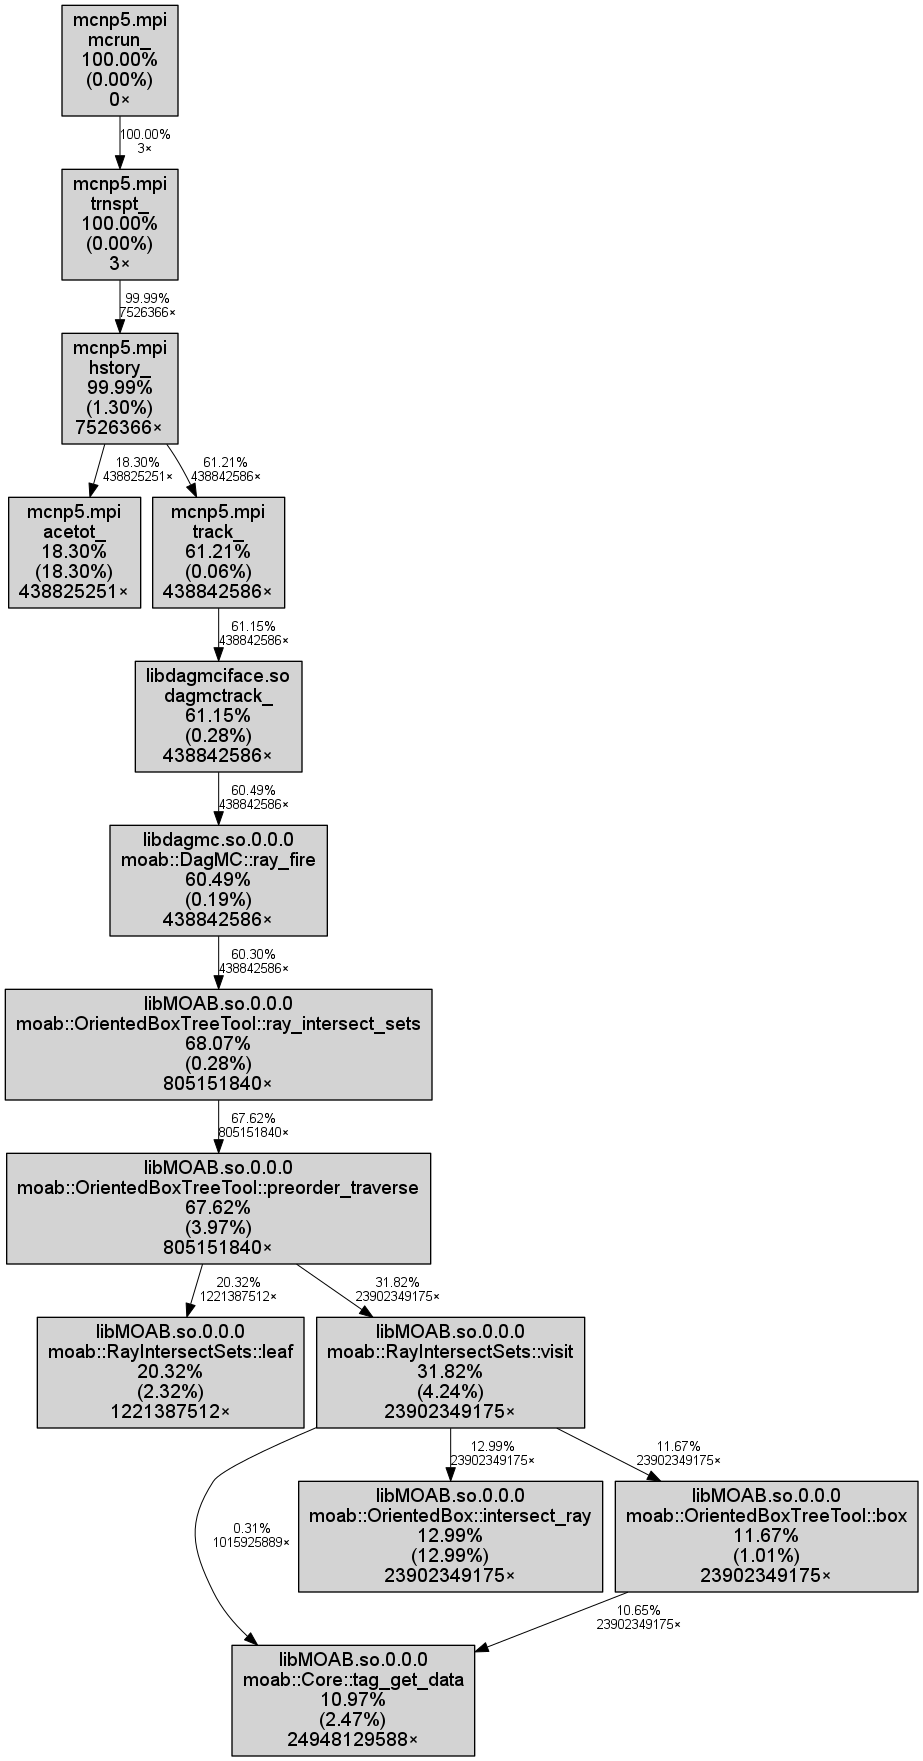
\includegraphics[scale=0.33]{dagmc_fng_cg_coarse.png}
\end{figure}

\begin{figure}[H]
  \centering
  \caption{Callgraph of native MCNP FNG run for 1E7 histories. (Processes taking $<$10\% of the runtime are filtered out in order to simplify the call graph.)}
  \label{mcnp-fng-coarse}
  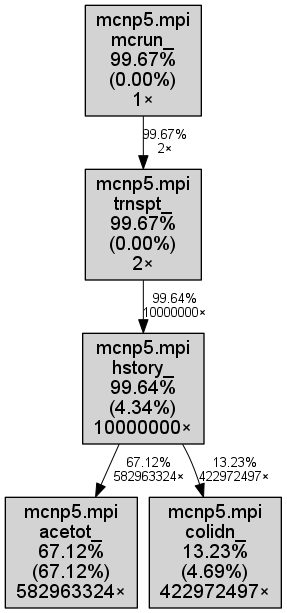
\includegraphics[scale=0.35]{native_fng_cg_coarse.png}
\end{figure}

The combination of the profiling results indicating how much time is spent in tracking particles in DAGMC along with the difference in absolute run times confirms that indeed the performance bottleneck of DAGMC lies in its ability to quickly satisfy the geometric queries of the underlying Monte Carlo code it is coupled to. Looking more closely at the underlying calls in DAGMC, one can see that this time is collectively spent in the DAGMC \textit{ray\_fire} call with the BVH traversal lying below this along with many underlying MOAB database-related calls. This indicates that this time is spent even more specifically in traversing MOAB's OBB BVH via the database-oriented methods available in DAGMC.

Again, it should be addressed that in this case a pre-built BVH was include in the geometry file and read into place much more quickly than in a typical DAGMC run. While this processes does contribute to additional DAGMC runtime, the amount of time spent building these hierarchies is small relative to the time spent in particle transport due to the high number of histories required for good statistics.


\subsection{High Valence Vertex Study}%%Status:In Progress%%
\label{hv_study}

It has long been suspected that one of the bottlenecks in DAGMC is ray tracing performance degredation in regions with high-valence vertices. High valence vertices are defined as those connected to an unusally high number of triangle entities. This region of the mesh will take on a fan-like shape as seen in Figure \ref{hv_examples}. High-valence vertices are known to occur on planar surfaces bounded by a circular curve. These regions are commonly generated in the faceting algorithms used to produce DAGMC meshes. This faceting scheme (which comes from ACIS libraries underlying the CUBIT/Trelis graphics engine) is designed to produce the smallest number of triangles possible to represent the model within the representation tolerance specified in DAGMC's surface mesh generation preprocessing. The faceting is produced this way because it is favorable to the rasterization process commonly used to display models interactively in the CAD program. Fewer triangles are better for the purpose particle tracking in DAGMC as well. Even the ideal ray tracing acceleration structure queries for a given triangle mesh scale as $O(log(N))$, and the size of models being analyzed using the toolkit provides motivation to keep memory footprints as low as possible. However, even with fewer triangles undesirable configurations can impede performance as is shown by a set of tests conducted on models generated using this faceting scheme.

A study by Steve Jackson in 2010 on the performance of the MOAB ray tracer revealed a steep degredation in performance with a decreasing faceting tolerance and an increasing number of triangles. Using a DAGMC-based ray fire test program, the performance of DAGMC's ray fire ability was evaluated for four models. These models include a simple sphere, a notched or slotted sphere, and an outer volume of an ITER model.

\begin{figure}[H]
  \begin{center}
  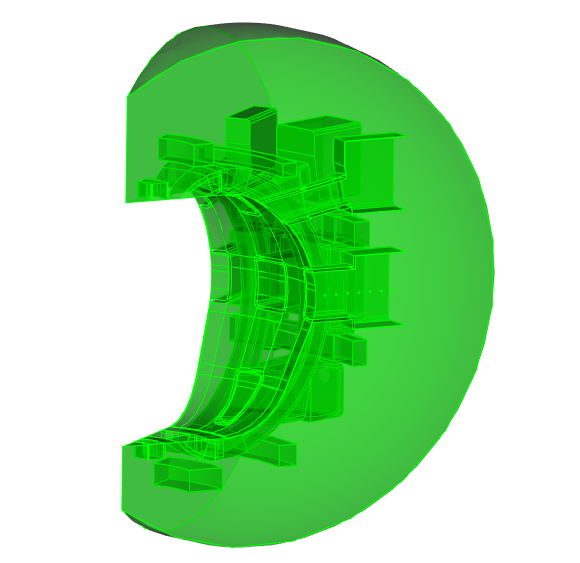
\includegraphics[scale=0.4]{iter_rf_vol.png}
  \caption{ITER volume used for ray fire testing.}
  \label{iter_rf_vol}
  \end{center}
\end{figure}

\begin{figure}[H]
  \begin{center}
    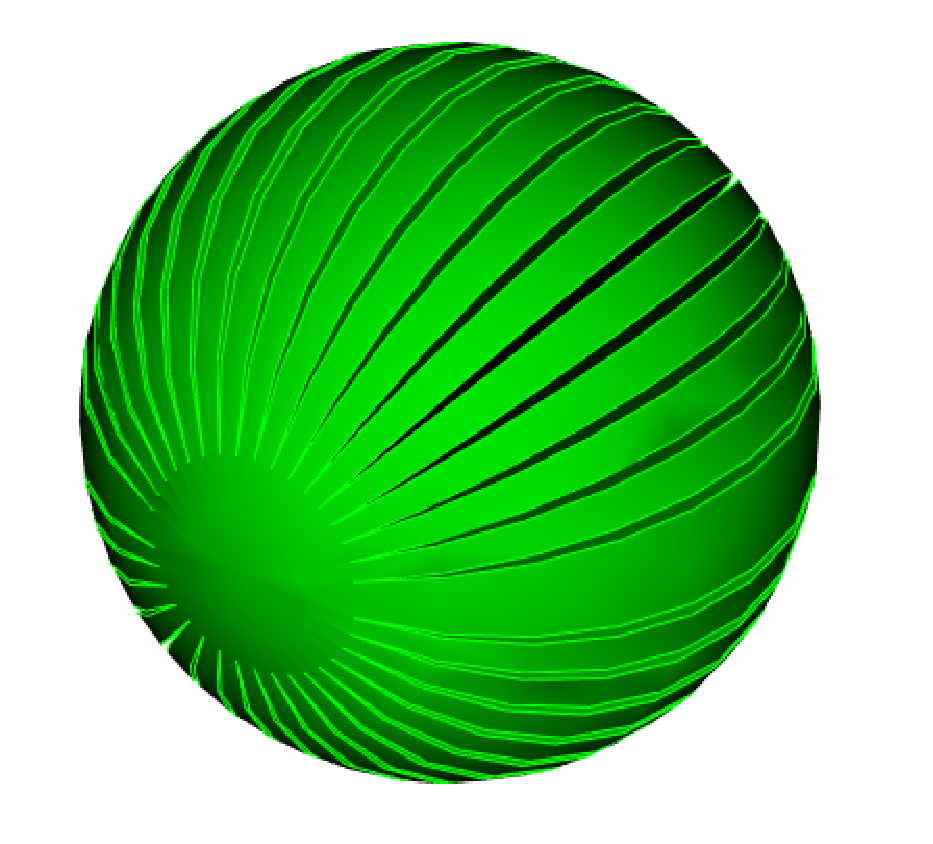
\includegraphics[scale=0.25]{ds.png}
    \caption{CAD representation of the slotted sphere.}
    \label{ds_cad}
  \end{center}
\end{figure} 

Each model presents its own challenges with increasing faceting tolerance. The sphere is a good control case for an increasing number of triangles without change in complexity. The number of triangles generated in the spherical case will tend toward a maximum value with decreasing faceting tolerance, but the general nature of the triangulated surface (triangle density, structure, etc.) will remain the same. This is not true of geometries with planar surfaces which may be able to be resolved exactly using some finite number of triangles making the sphere a vaulable test model in that regard. In the case of the notched sphere, high-valence regions are generated by the faceting engine as a result of its underlying algorithms for planar surfaces meeting curves surfaces. The high triangle density of high valence regions cause overlaps in bounding volumes which become exacerbated as the faceting tolerance decreases. This results in inefficient hierarchy traversal. Additionaly, and perhaps more importantly than the presence of high valence regions, rays being fired with a point of origin at the center of the model causes them to travel either exactly along or very near to the surfaces of the planar slots in the sphere. Such a ray query will visit many internal nodes of the hierarchy during traversal, creating what is referred to as a very wide traversal as opposed to a narrow traversal in which fewer branches and fewer nodes of the tree are visited. In this way, the slotted sphere provides a good measure for the performance of a wide traversal through the hierarchy in a situation for which many of the internal nodes are required to be visited. Finally, the faceting of a volume from an ITER model is used. This volume comes from a real world application of DAGMC's ray tracing kernel and is also known to contain high valence regions as well (see Figure \ref{hv_examples}).

In each of these tests, the models are tesselated with an increasingly smaller faceting tolerance resulting in a higher number of triangles and more complex nature of the surface mesh in terms of BVH construction and traversal. The faceting tolerance being defined as the maximum distance between the faceted curve or surface and the geometric curve or surface which it resolves. 

\begin{figure}[H]
  \begin{center}
    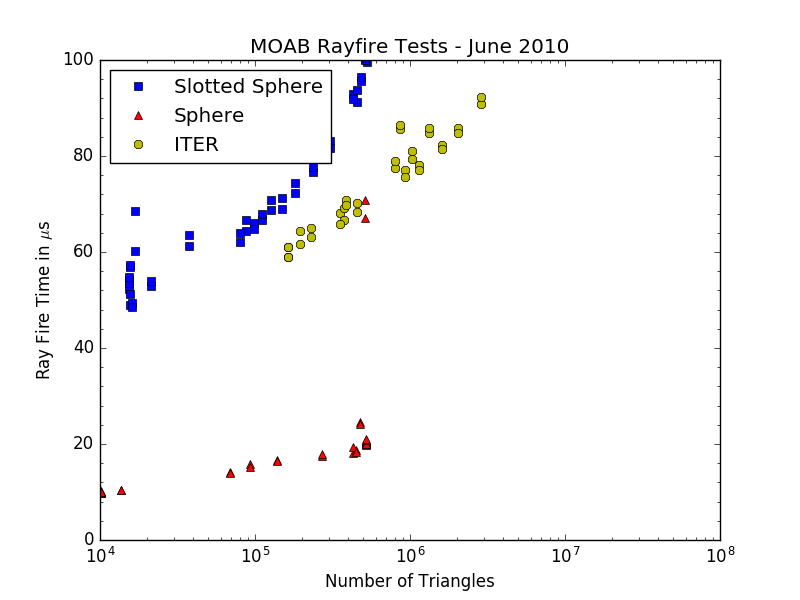
\includegraphics[scale=0.5]{SJ_tests_2010.png} \\
    \caption{Results of MOAB ray tracing performance tests with decreasing faceting tolerance performed by Steve Jackson in June of 2010. Data points represent average time spent in firing a ray.}
    \label{sj_tests}
  \end{center}
\end{figure}

While the sphere model shows good scaling with increasing number of triangles, the ITER volume and slotted sphere both have a pronounced increase in average ray fire time with decreasing faceting tolerance. Knowing that both of the latter models contain high valence regions, it was postulated at the time that these regions had a significant effect on the scaling. In order to isolate the high-valence vertex problem generated by the ACIS graphics faceting algorithm, a manually generated mesh was generated in MOAB with an artificial high-valence region (shown in Figure \ref{hv_cube_design}). This mesh is a modified cube centered on the origin in which the typical two-triangle faceting has been replaced by a more complex planar surfce of triangles including an interior high-valence region within the face. The high-valence region was generated by inserting vertices along the diagonal of the interior box and connecting them to the opposing corners of the box. This construction was designed such that the valence of the corner vertices in the interior region could be controled along with the size of the interior region relative to the size of the entire face. Tests were then peformed by varing these two parameters in order to characterize the performance impediment based on these two factors and to determine its root cause.

\begin{figure}[H]
  \centering
    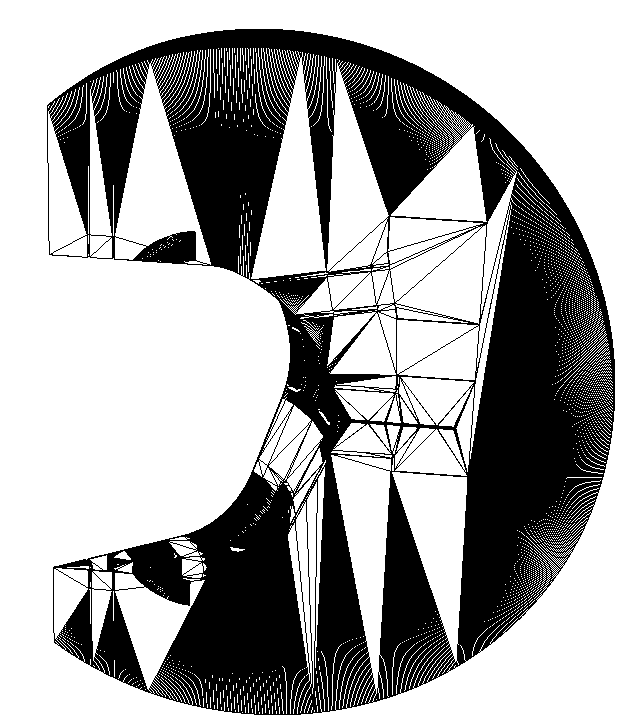
\includegraphics[scale=0.2]{iter_sideon.png}
    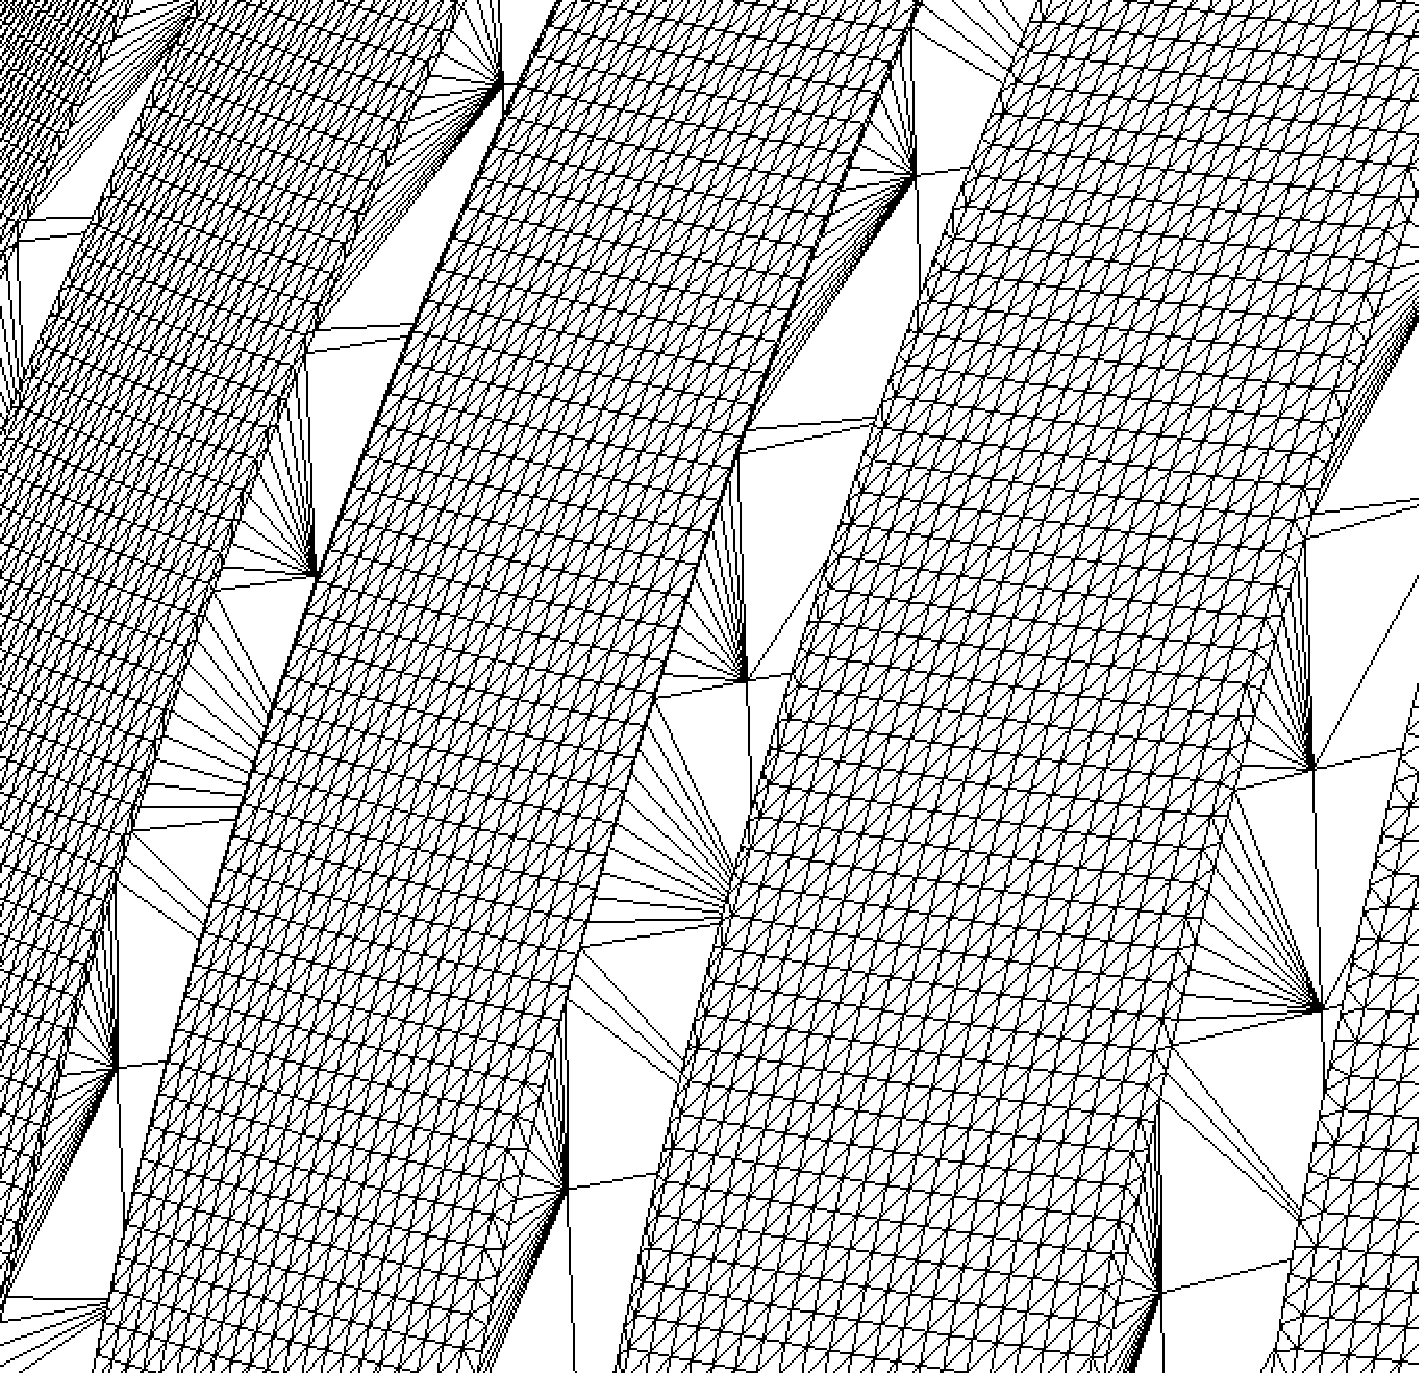
\includegraphics[scale=0.1]{ds_hv.png}
    \caption{Exampels of high valence regions in analysis and test models.}
    \label{hv_examples}
\end{figure}

A simple ray fire test program was used to construct ray tracing acceleration structures and conduct ray queries using DAGMC's interface in the same way as it is done during particle transport. Information on this test program can be found in the appendix of this work. This program was used to fire rays with random direction from the origin of the test model while directionally biasing the rays such that they should always find intersections on the modified surface containing the high-valence region. Many tests were done while varying the percentage of the surface covered by the high-valence region as well as the valence of the region. Specification of the random number seed is allowed within the program, giving a more direct comparison of performance with the gaurantee that the same set of rays is fired in each test case.

\begin{figure}[H]
  \centering
    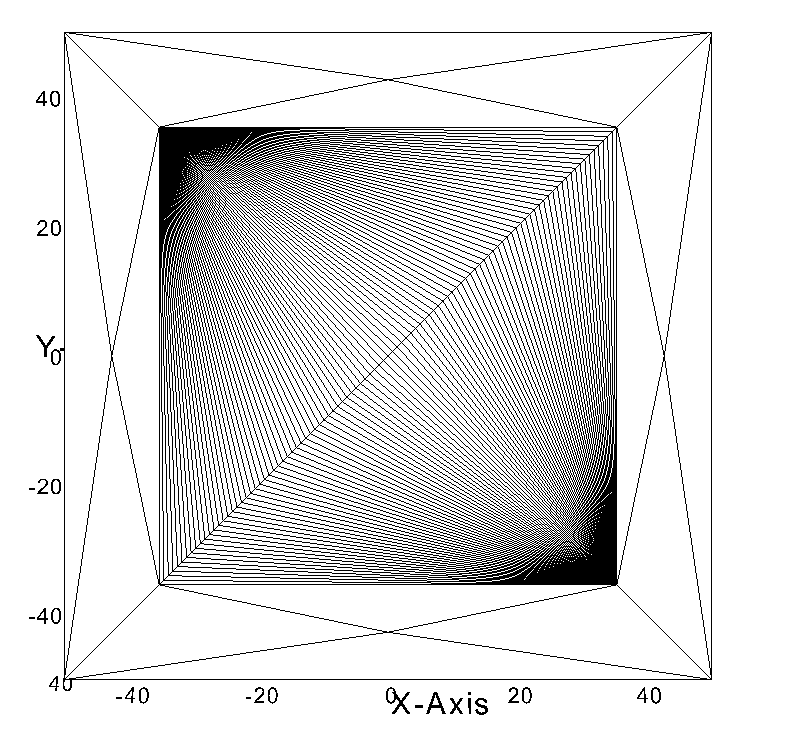
\includegraphics[scale=0.33]{hv_study_design.png}
    \caption{Side-on view of the modified cube mesh used to study the high-valence vertex problem.}
    \label{hv_cube_design}
\end{figure}

All of the following tests vary the valence of the corner vertices from 2 to 50,000 and the fraction of the surface covered by the high valence region from 0 to 1. From what is known about the nature of the BVH used in DAGMC, it was expected that ray fire times increase as the area fraction increases becuase rays are more likely to enter the high valence region. It was also expected that as the valence increases ray tracing speed would decrease due to what is already known about a high-valence region's effect on the ray tracing speed. However, these results meet only one of those expectations. The ray fire times become worse for an increase in valence, but for a given valence a lower area fraction actually shows a much longer ray fire time than the larger area fractions. This suggests that the presence of a high-valence region in a surface could be causing problems in building and traversing the BVH no matter the relative area of the region. In order to investigate this matter further a visualization tool was developed to view MOAB's oriented bounding boxes as constructed by MOAB's building algorithm.

\begin{figure}[H]
  \centering
    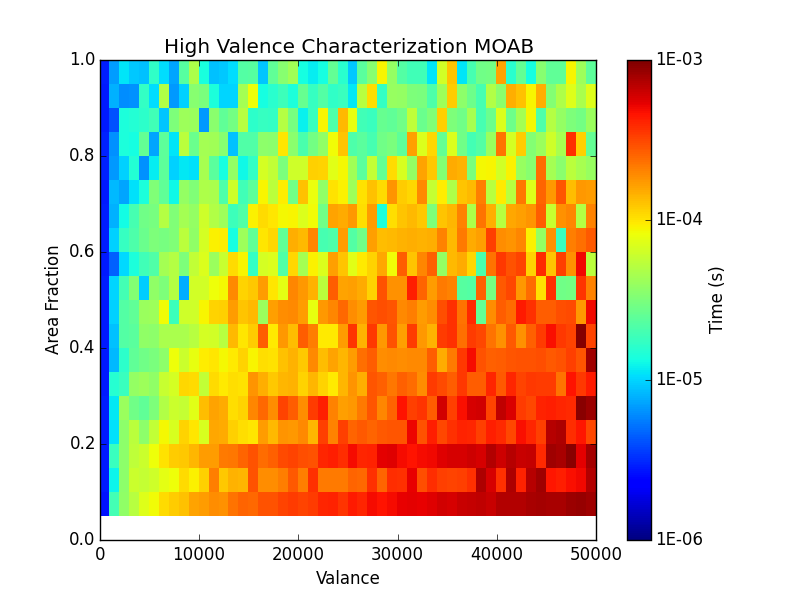
\includegraphics[scale=0.55]{hv_study_MOAB.png}
    \caption{Results from parameter sweep of valence and valence area fraction in the high-valence test mesh.}
    \label{hvsideon}
\end{figure}

Using a visitor pattern in the BVH, each oriented bounding box was converted into a MOAB hex element and saved on a new mesh instance and written out for examination. Each box  element was additionally tagged with it's depth in the tree as well as the triangle entities that it contains if it represents a leaf node. This program then outputs a mesh which can be used to visualize the BVH level by level on top of the geometric mesh. At lower depths in the BVH, only bounding boxes in the high valence region are present. This is expected in that it will take more bounding boxes and therefore a deeper tree in that region in order to resolve the larger number of triangles into smaller sets and eventually reach leaf conditions. An important observation in this region was that the bounding boxes of the high valence surface often contained some portion of the high valence region's triangles as well as other triangles in the modified surface. Often bounding boxes such as these were found to be leaf nodes of the tree (Figure \ref{bad_hv_box}). Not only is this a problem in the sense that it implies a large number of triangle checks will be necessary if this leaf node is hit, but if this leaf node also contains triangles outside the high valence region with large area as we tend to see in this model, then  the leaf becomes much more likely to be traversed, even though the chances that the ray is going to hit a triangle in the high valence region is relatively small. In this way the default building algorithm creates an artificially high cross-section for high-valence leaf nodes by containing adjacent triangles to that region.

\begin{figure}[H]
  \centering
    \includegraphics[scale=0.3]{{obbs_wsr_0.95}.png}
    \caption{View of culprit bounding box containing many high valence region triangle as well as other surface triangles. Blue box and triangles: leaf node bounding box and associated triangles. Red boxes: Other representative boxes at the same depth in that tree.}
    \label{bad_hv_box}
\end{figure}

MOAB's BVH building algorithm employs a median splitting method governed by a set of parameters use to determine if a node split is considered advantageous by the building algorithm. One metric heavily favored by the algorithm is the splitting ratio of the resulting child boxes for a given splitting plane. The splitting ratio of a given node is defined by the absoulte difference in the entities between the child nodes divided by the total number of entities in the parent node. When building a BVH, MOAB sets a best and worst case value for this splitting ratio. If the splitting ratio for a given splitting plane is found to be better (smaller) than the best case splitting ratio then the node is split and the recursive top-down build continues. If the splitting ratio for a given splitting plane is worse than the worst case splitting ratio, then the node is not split to avoid overly large/deep trees and large overlaps in sibling bounding boxes. If the splitting ratio is found to be between these two values, the ratio is tracked as further candidate split planes are tested. When all splitting planes for the box axes have been checked, the child entity lists with the best splitting ratio is then used to perform the split.

In this case, the parameter of interest is the worst case splitting ratio. This parameter is intended to keep trees from becoming too deep by avoiding node splits which do not effectively divide entities. The default setting for the worst case split ratio is 0.95. In the case of the high valence vertices, many of the entities are packed tightly together, meaning that as the valence increases for a given area fraction, the splitting ratio will become worse and worse with splitting planes that are unlikely to divide these entities in a way that is seen as an acceptable split criterion by the building algorithm. Additionally, as the high valence region grows smaller relative to the surface size, this problem is only exacerbated in that the high valence region triangles become more closely packed together and less likely to be split by a median plane. The triangles exterior to the high valence region become larger relative to the area of high valence triangles contained by the node, causing the artificially high cross-section of the high valence region to be come larger as well.

\begin{figure}
  \begin{align*}
  splitting\;ratio  = \dfrac{|left\; child\; primitives\; -\; right\; child\; primitives|}{parent\; entities}
  \end{align*}
  \caption{Description of MOAB's splitting ratio heuristic used to construct its oriented bounding box BVH.}
  \label{split_ratio}
\end{figure}

  Fortunately MOAB allows one to have control over the parameters used to govern the BVH building algorithm. By altering this parameter, we can study its effect on the quality of the BVH and its adaptability to the high valence region. In addition to the valence and area fraction of the high valence region, the worst case split ratio was explored as well for values ranging between 0.95 and 1. The hypothesis here being that forcing the algorithm to continue splitting regardless of a poor splitting ratio on the number of entities would break up these prematurely ended branches in the BVH and eventually split up the high valence region as well. Upon reaching the same condition as before in which a box contains many of the high valence region triangles as well as a few triangles exterior to that region, increasing the worst case splitting ratio will force the algorithm to split the node. Even if this initial split, and other subsequent splits like it, seem disadvantageous at first this will gauarantee that the high-valence region will eventually be partitioned properly by the BVH. After some experimenting with new values for this parameter, the results were quite promising.

  \begin{figure}
    \centering
    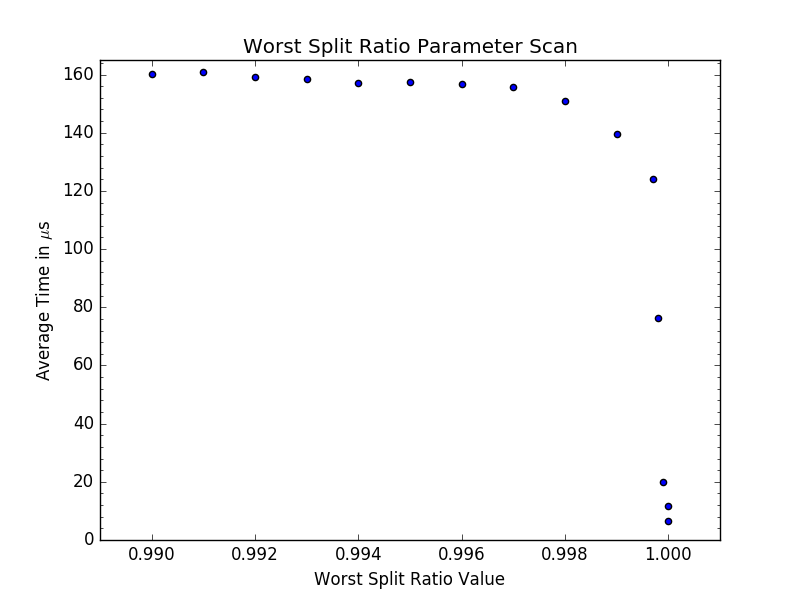
\includegraphics[scale=0.55]{wsr_scan.png}
    \caption{An average of the average ray fire times for hv study sweep when scanning the worst splitting ratio parameter from 0.98 to 1.}
    \end{figure}
  
  The test results for changes in this parameter show little change until the worst case splitting ratio reaches 1. This demonstrates the magnitude of the  perturbation the high valence region causes in the BVH building algorithm. However, when this parameter reaches 1, the maxiumum value possible for the splitting ratio, the BVH builder is effectively forced to continue splitting until a new stopping criterion is met. This new stopping criterion is the minimum number of entities allowed in a single leaf. This value is based on an estimation of the number of ray-triangle intersection checks that can be done in the amount of time it takes to do a ray-box intersection check. MOAB's BVH builder uses a default value of 8 for the minimum number of triangles allowed in a leaf node. The results of the same ray fire tests on the hv model using a worst case splitting ratio of 1 and an effective leaf criterion of a minimum number of entities are below.

  
\begin{figure}[H]
  \centering
    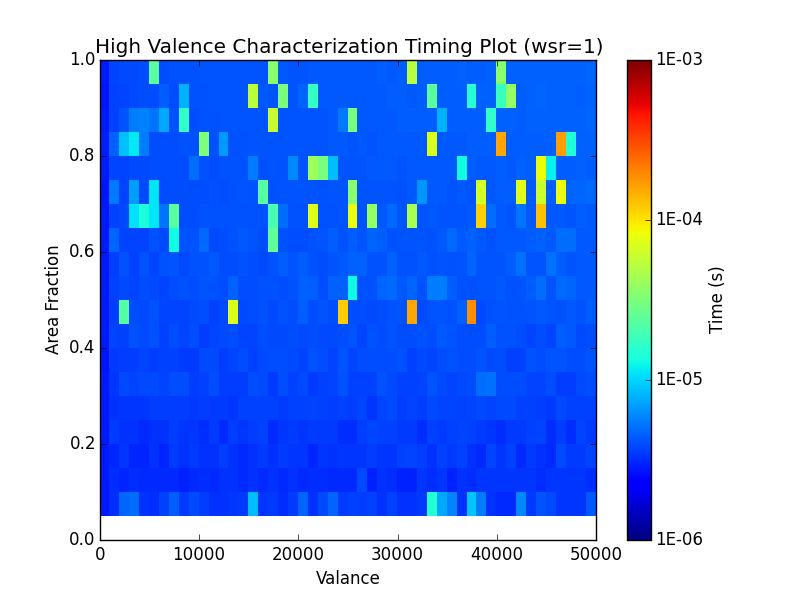
\includegraphics[scale=0.55]{hv_study_MOAB_wsr1.png}
    \caption{Run of the high valence characterization study with a worst case splitting ratio set to 1.}
\end{figure}


With this small change to the BVH builder's parameters, performance with a high valence region becomes significantly better. This change is likely unsuitable for the general case of a tesselated surface however. A default worst case splitting ratio value of 1 will lead to much deeper trees which on average, will take longer to traverse as a result, and will consume more memory. However, altering this paramter by identifying high-valence regions could greatly improve particle tracking performance as these regions appear in many meshes generated using the DAGMC workflow.


\subsection{Linking DAGMC with Intel's Embree}%%Status:In Progress%%
\label{emdag}

As discussed in Section \ref{perf_benchmark}, a number of MOAB-related database calls appear in the profiling of a DAGMC run. MOAB is a powerful tool for mesh manipulation, analysis, and storage, but the implementation of an efficient ray tracer in the context of this database design inherently comes with a large amount of overhead. As a result, an attempt at the replacement of MOAB's ray tracing system with a highly-optimized ray tracer was made. Recently, Intel has made an effort to produce just such a CPU-based raytracer called Embree \cite{Wald_2014}. In both construction and traversal of BVHs, Embree takes advantage of many of the latest developments in BVH research by using modern chipset architecture capabilities via vectorization at an implementation level as described in Section \ref{subsec:accel_datastructures} of this work. The combination of these effects leads to a very powerful raytracing tool in terms of performance. As a result of these factors, Embree was chosen as the tool to be applied in DAGMC to satisfy geometric queries for MCNP. The resulting combination of these tools will be reffered to as EmDAG for the remainder of this section.

\subsubsection{Transferring DAGMC Model's to Embree Scenes}%%Status:Done%%

The process of employing Embree as DAGMC's ray tracer begins by establishing an equivalent representation of the MOAB mesh in Embree. In comparison to MOAB, Embree is limited in its ability to represent the underlying topological structure of a model. This topology is necessary and used advantageously during particle tracking in DAGMC by reducing the set of triangles queried to those of the particle's current volume and thus reducing the number of point containment queries. However, a method was discovered to represent enough of the topology to meet the requirements of DAGMC transport. The highest level representation in Embree is referred to as a scene. Each scene may contain one or more geometries or triangle surface meshes. Fortunately, this system is enough to create a workable representation of DAGMC meshes in which MOAB volumes are the equivalent of Embree scenes and MOAB surfaces are represented in their respective scenes as surfaces. This method provides a one-to-one mapping of MOAB volumes and surfaces to their corresponding entities in Embree and allows all topology-based operations to proceed inside of DAGMC in their usual manner. In this way, the requirement for topological information in DAGMC at the surface and volume level is met. Next, transfer of the primitive mesh data is considered.

Scenes do not share mesh data as volumes are able to do in MOAB, so the triangle connectivity of each surface is reproduced in each scene they belong to. Fortunately, Embree does allow the sharing of vertices between scenes. In order to take advantage of this feature, all of the vertices in the MOAB mesh are provided in the Embree instance as a global vertex buffer. Surfaces from all scenes can then be defined by a connectivity of vertices from this global pool of points. This method guarantees that the each surface can be represented by the same set of stored vertices in each scene it belongs to giving the exact same representation in each scene. It greatly simplifies particle tracking by guaranteeing that the same surfaces will not overlap each other in the different scenes they are a part of by doing the conversion of points from the MOAB database to Embree only once. Additionally, this method will maintain watertightnes at the boundaries between surfaces ensuring the same model fidelity as the representation in MOAB.

\begin{figure}
  \centering
  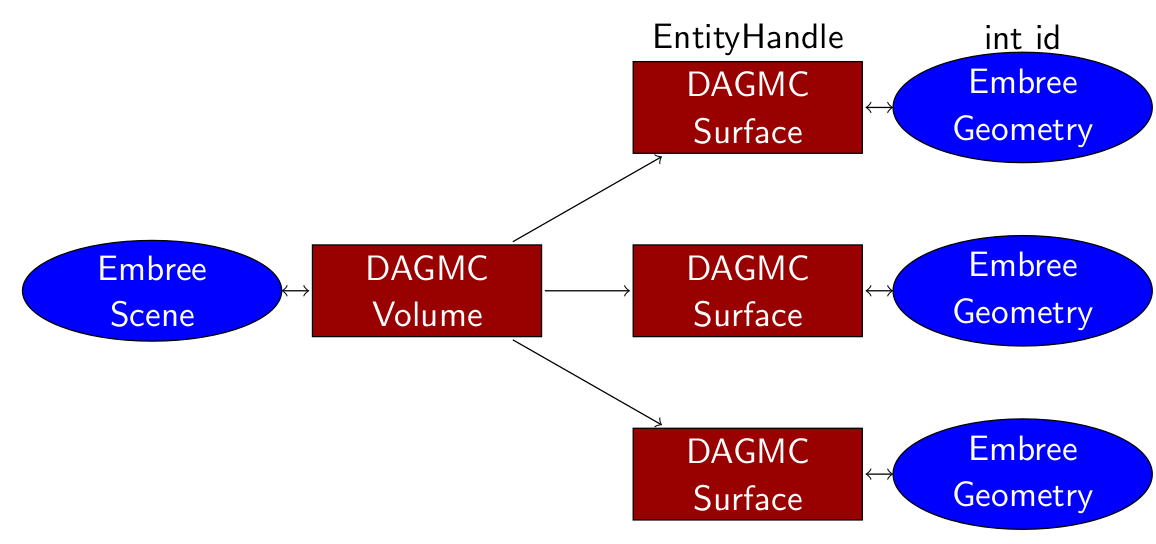
\includegraphics[scale=0.3]{emdag_mapping.png}
  \caption{Representation of MOAB tracking topological connections while mapped to Embree to perform ray queries.}
  \label{emdag_mapping}
\end{figure}

The representation of triangle normals are important to the DAGMC particle tracking algorithm established by Smith et. al. in 2011  \cite{Smith_2011}. In DAGMC, particles on or just outside the surface of a volume are handled by ignoring the near-surface intersection upon being established in a new volume. This is done to maintain tracking of particles based on their logical position in the model rather than solely their numerical position which can cause ambiguities regarding point containment and cause lost particles or trapped particles between surfaces with infinite histories. Logical particle tracking is implemented using the convention that triangle normals will always point outward from the center of the volume they belong to. Triangles hit by the ray are ignored if the normal of the triangle opposes the ray direction via a dot product calculation to ensure only exiting ray intersections are considered. While this has historically been handled inside of DAGMC, this is accomplished in EmDAG via the use of Embree's filter functions. Filter functions allow for a user-defined callback method which allows users to validate a ray hit inside of Embree before returning a final result. Embree will return its most recent intersection with the scene to the filter function (the hit triangle's unnormalized vector included) and allow a method to either accept the hit or instruct Embree to continute tracing the ray path based on the outcome of the filter function. In MOAB, triangle normals are set in a global manner and adjusted using stored information within MOAB based on what volume is being queried at the moment. This is referred to as the surface's sense with respect to that volume. Because we are forced to duplicate surfaces in Embree, the triangle normals are pre-oriented based on this surface's sense for the scene it is being created in upon initialization of the model within the Embree instance. This saves steps in gathering this information upon traversal when the triangle normal is needed to determine a particle's logical position within the model. Though the connectivity of triangles is duplicated using this approach, the overall memory footprint of EmDAG after duplicating the DAGMC geometry in Embree is not much greater thanks to the single precision values for vertex locations used in Embree which will be addressed in a later section of this chapter.
By meeting DAGMC's requirements in the areas of topology, watertight representation, and hit acceptance/rejection based on triangle normals, Embree provides DagMC with all the information needed to perform geometric operations required by the various Monte Carlo codes it supports, but in an agnostic manner to the ray tracing kernel being used.

\subsubsection{EmDAG Performance Testing}%%Status:In Progress%%

Using the same DAGMC-based ray fire test program, the performance of DAGMC's ray fire ability was compared to that of EmDAG's for three models. These models include a simple sphere, a notched sphere, and a high aspect ratio cylinder. In each of these tests, the models are tesselated with an increasingly smaller faceting tolerance in a higher number of triangles and more complex nature of the surface mesh in terms of BVH construction and traversal. The faceting tolerance is defined as the maximum distance between the faceted curve or surface and the geometric curve or surface which it resolves. 600k rays are then fired from the center of the volume isotropically using the same random number seed so that the same set of rays is fired in each ray tracing system.

\begin{figure}[H]
  \begin{center}
    \begin{tabular}{ccc}
      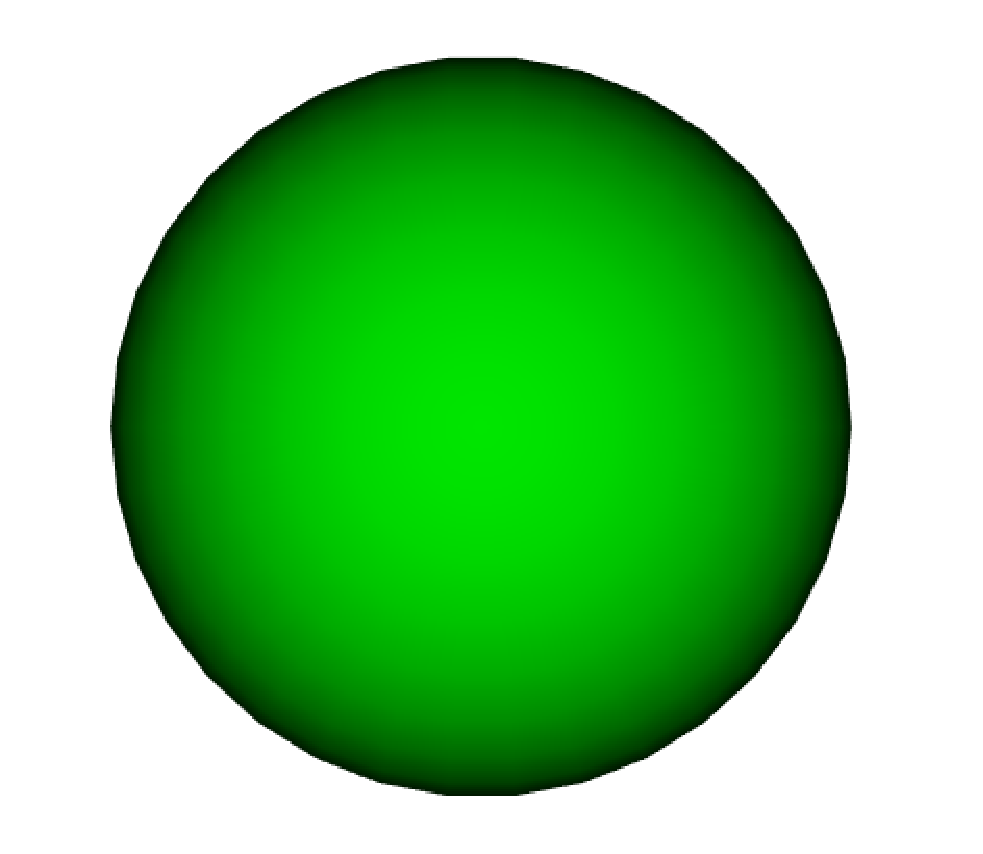
\includegraphics[scale=0.13]{sphere.png} &
      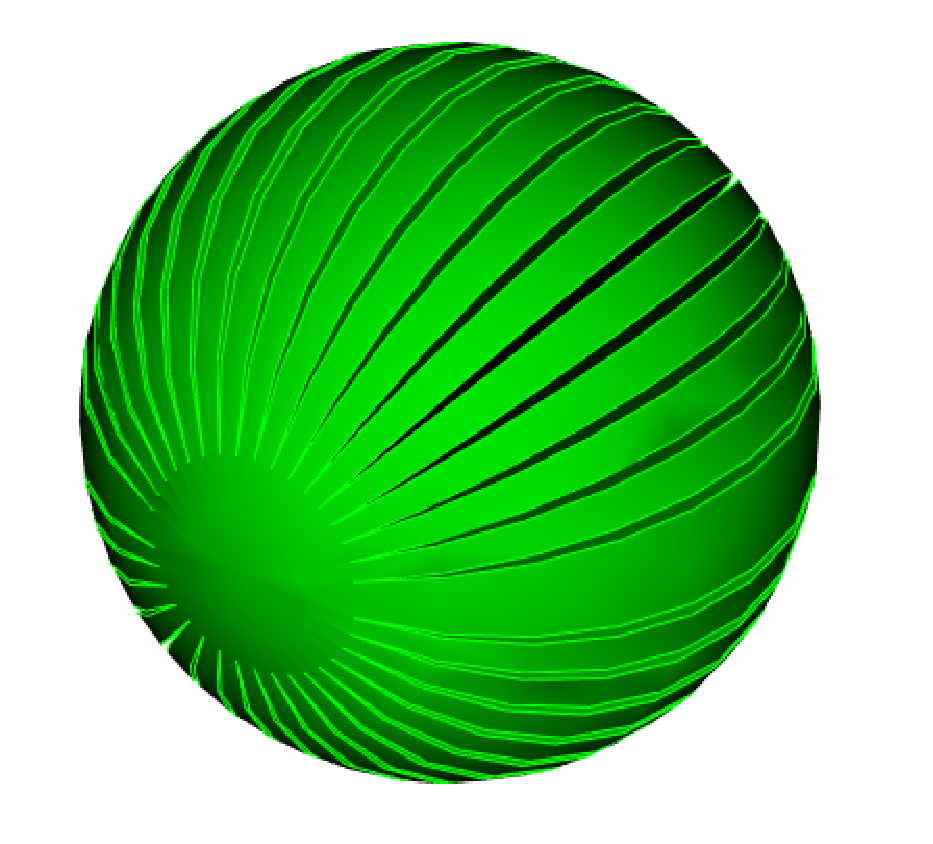
\includegraphics[scale=0.13]{ds.png} &
      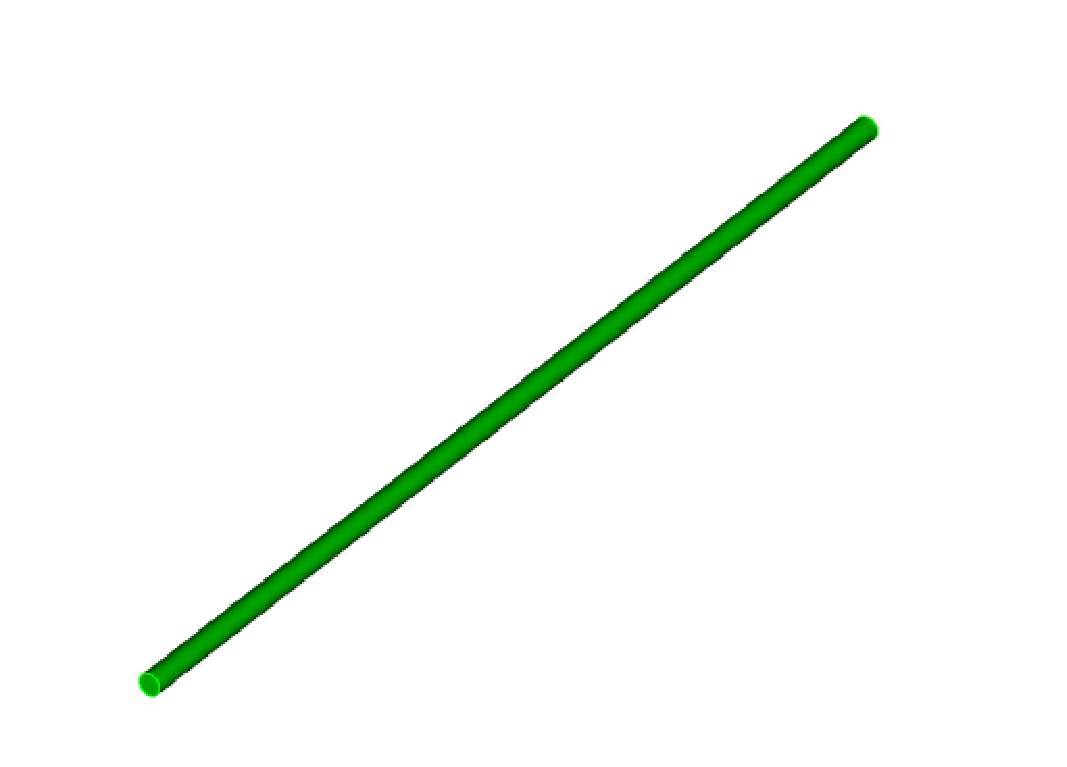
\includegraphics[scale=0.13]{larcyl.png} \\
    \end{tabular}
    \caption{CAD representations of the sphere, slotted sphere, and high aspect ratio cylinder test models used for ray fire timings of DagMC and EmDagMC. (left to right) \label{models}}
  \end{center}
\end{figure} 


The sphere and slotted sphere models present speicalized challenges to the BVH datastructure as described in Section \ref{hv_study}. Due to memory contraints of the system used for testing EmDAG's performance against DAGMC, the ITER volume was removed and replaced with a high aspect ratio cylinder. The faceting of the cylinder contains many long, thin triangles running along the barrel of the cylinder. In similar fashion to the spherical model, the number of these triangles will increase with decreasing faceting tolerance resulting in an increasing triangle density as well. The low aspect ratio nature of these triangles can cause difficulty in the calculations of tightly fitting OBBs within MOAB's BVH builder. This test model is used to the ray tracing systems robustness of the BVH generation algorithms to objects with surface meshes of this nature.

The standard DAGMC ray fire test program (included in appendix A) was used to evaluate both ray fire systems. The test program itself is agnostic to the underlying ray tracing kernel used by DAGMC and two versions of the program were compiled. One in which DAGMC uses MOAB's ray tracer and another in which MOAB's ray tracing system is subverted by Embree, a.k.a. EmDAG. The two sets of timing results can be found in Figure \ref{emdag_timing_compare}.

\begin{figure}[H]
  \vspace{-3cm}
  \centering
  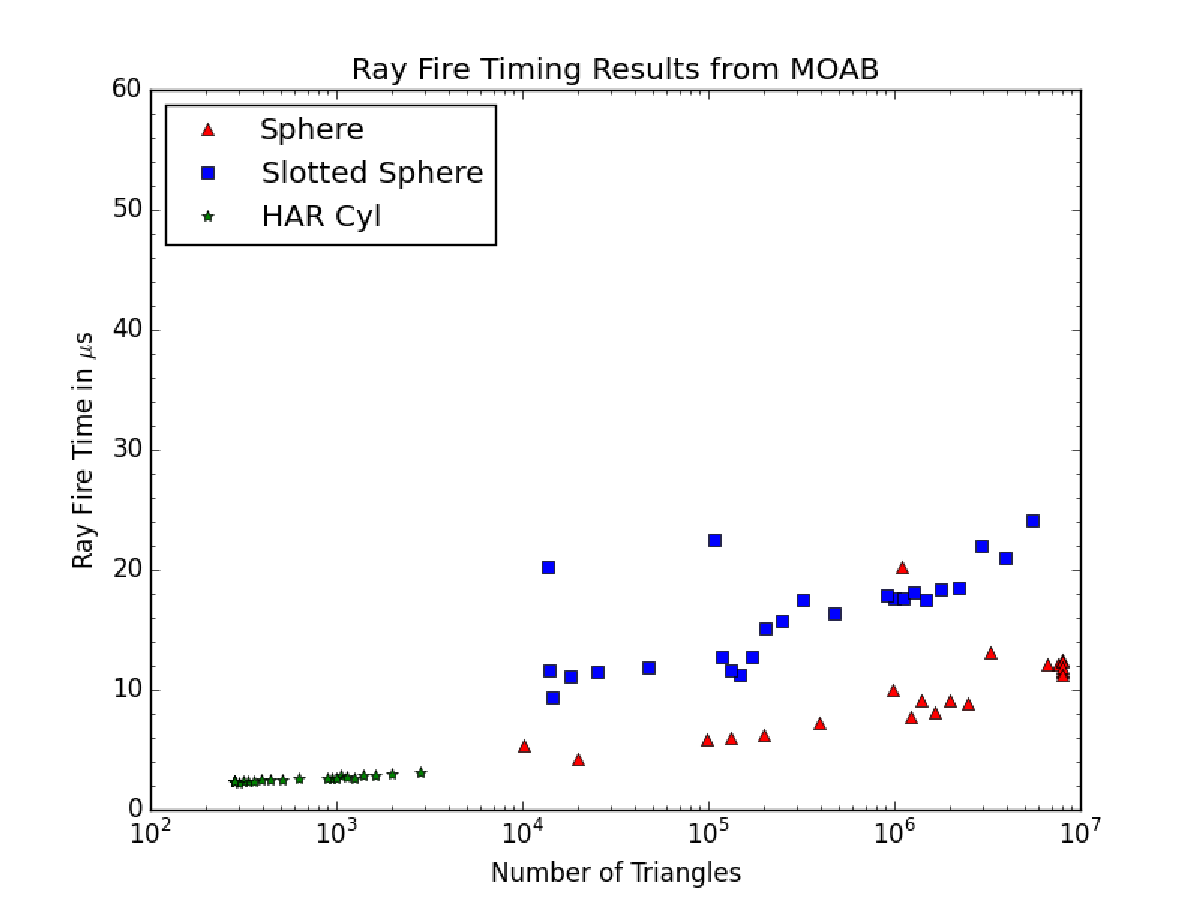
\includegraphics[scale=0.33]{Eig_fix_rf.png}
  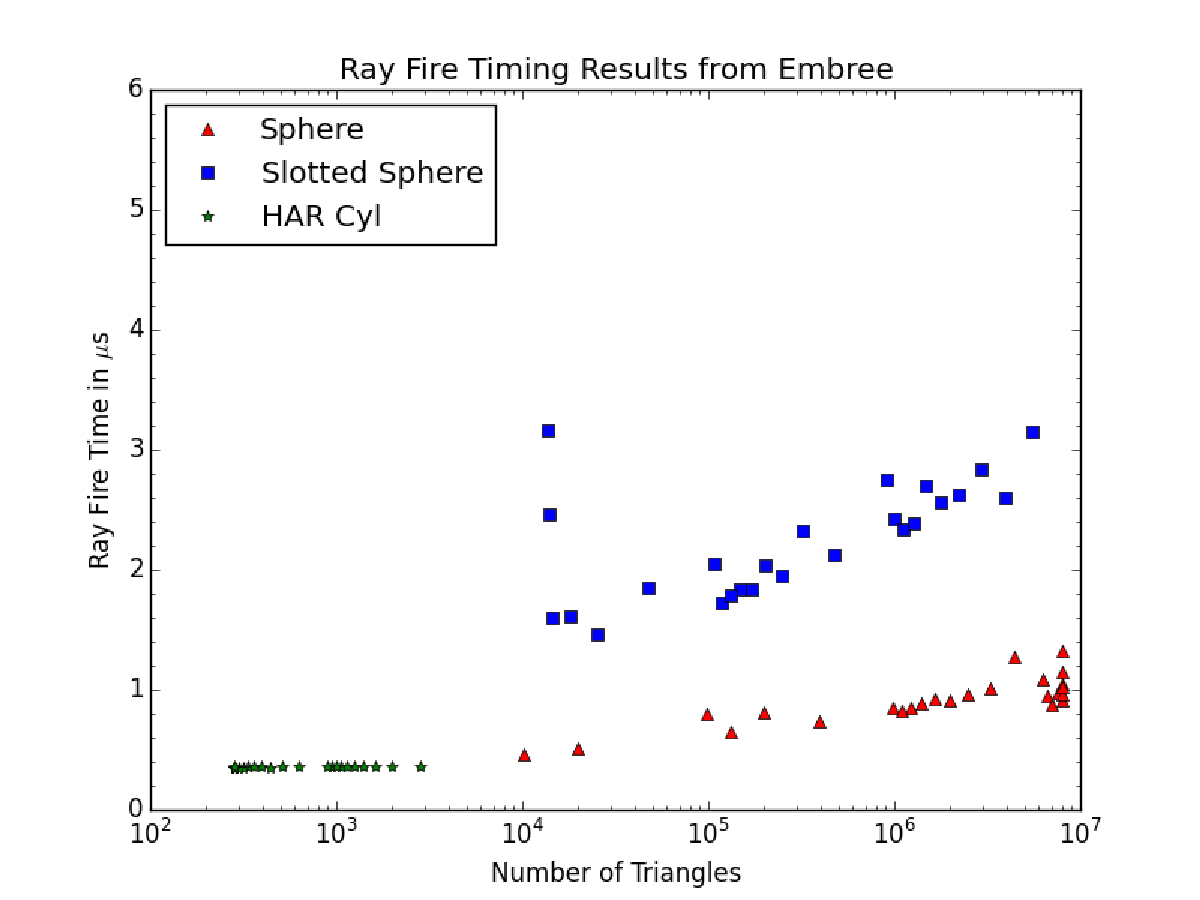
\includegraphics[scale=0.33]{embree_rf.png}
  \caption{A comparison of average ray fire times between DAGMC using MOAB's ray tracing and Embree. Please note the difference in time scale.}
  \label{emdag_timing_compare}
\end{figure}
\newpage

%The results of these tests validate the suspicion that the MOAB database contains a considerable amount of overhead for the implementation of a ray tracing kernel. This is indicated in the way that the ray tracing times scale for each model in both kernels.
Both MOAB and EmDAG scale relatively well for the HAR cylinder model with decreasing faceting tolerance. This indicates that both systems are capable of building bounding volumes well for a model with long, skinny triangles. The scaling of the spherical case with increasing triangles is slightly worse than the HAR cylinder most likely because the BVH tree is unavoidably going to becomce gradually deeper as more and more triangles exist in the model. Finally, the slotted sphere contains many high valence regions and as expected it scales the worst with decreasing faceting tolerance as the valence of these regions increases. It is very apparent that there is nearly an order of magnitude difference in the ray fire timings MOAB and Embree. Due to the very similar scaling of each test model, it can be stated that the majority of the descrepancy in the ray fire timings between the two systems occurs in the traversal methods employed by both systems and isn't likely due to a significant difference in the structure of the BVH being built by either system. Changes in the way the BVH is built typically accounts for anywhere from 30-40\% difference in ray fire timings whereas the descrepancy seen here between MOAB and Embree is on average \textbf{an order of magnitude better} when using Embree. In large part, this has to do with Embree's freedom of design without the restriction of a ray tracing implementation inside the context of another application. MOAB's flexibility in core design allows for the robust implementation of an oriented bounding box tree within this context, but comes with the overhead of database calls to retreieve stored information which can be undesirable for a high-performance system and doesn't allow MAOB to take advantage of some implementation optimizations that Embree does. The vectorization of Embree's traversal through its BVH contributes greatly to its speed. This can be also considered a part of the design freedom allowed when designing an independent ray tracing system that cannot not be afforded using only MOAB's database interface. However, a property unique to MOAB may allow for an implementation such as this as will be discussed near the end of this work.

\subsection{EmDAG Transport Tests}
\label{subsec:emdag_transport}

As an extension of these pure ray fire tests, the effect of an improved ray tracing system on particle transport was studied as well. These tests begin with several simple models and end with the application of EmDAG to one of the models used for DAGMC performance benchmarking in Chapter \ref{perf_benchmark}, FNG.

The first transport models to be tested were a single cube and single sphere filled with a dense hydrogen material for high collisionality in the problem resulting in a large number of ray queries in the transport run. Each of these models' principal dimension is 10 cm. The source for these models is a 5 MeV neutron isotropic point source at the center of the volume. One million particles were simulated in each test. All of the test models were preproccessed using a faceting tolerance of $10^{-4}$cm. Moving upward in complexity, another set of tests were run using a set of nested cubes and nested spheres. Each of the nested volume models contained three cells: the inner volume, a shell volume, and the graveyard volume. The purpose of these tests was to ensure that particles could in fact be tracked through multiple volumes robustly. The nested cubes model contains an extra volume which consists of the original single cube subtracted from a cube 1cm larger in each dimension. The nested sphere model contains an extra volume consisting of the original sphere from the single volume model subtracted from a sphere 1cm larger in radius. As the purpose of these tests was to test EmDAG's particle tracking between non-zero importance cells, the dimensions of the offset between the nested volumes is largely irrelevant so long as particles are in fact reaching all of the cells.

\begin{table}[H]
  \small
  \begin{center}

      \label{timings}
    \begin{tabular}{lccc}

      \toprule
      Test Model & MCNP & DagMCNP & EmDagMCNP \\
      %%\hline
      & \multicolumn{3}{c}{\textbf{time (min)/ ratio to MCNP}} \\
      \hline
      Sphere & 2.93 / 1.00 & 25.13 / 8.58  & 4.73 / 1.61  \\
      Cube & 5.03 / 1.00 & 10.56 / 2.10 & 5.80 / 1.153 \\
      Nested Spheres & 4.35 / 1.00  & 50.82 / 11.68  & 7.94 / 1.83 \\
      Nested Cubes & 4.73 / 1.00 & 9.26 / 1.96 & 4.35 / 0.92 \\
      %%\hline
      &  \multicolumn{3}{c}{\textbf{histories/min}} \\
      \hline
      Sphere & 3.4104E+05  & 3.9944E+04  & 2.1810E+05   \\
      Cube & 1.9879E+05 & 9.4738E+04 & 1.7260E+05 \\
      Nested Spheres & 2.2991E+05 & 1.9877E+04 & 1.3947E+05 \\
      Nested Cubes & 2.1170E+05 & 1.0806E+05 & 2.3026E+05 \\
      \bottomrule
      
    \end{tabular}
  \end{center}
  \caption{Runtime comparison native MCNP, DAG-MCNP, and EmDAG-MCNP over four transport test problems.}
  
\end{table}

The native MCNP runs were generally the fastest among the test problems with the exception of the nested cubes case in which EmDAG-MCNP marginally outperformed the native code by ~8\%. This is likely due to the fact that very few triangles are needed to exactly represent the surfaces of cubic volumes. This creates a very simple problem in the area of BVH building and results in a shallow tree. The fact that these volumes have multiple surfaces is also of importance here. MCNP searches linearly through a given cell's (volume's) surfaces to determine the intersection of a particle with the nearest surface whereas both DAG-MCNP and EmDAG-MCNP perform this search spatially. In the nested cubes model, it is likely that the number of surfaces relative to the number of triangles in their representation is high enough to allow EmDAG-MCNP to overtake MCNP's CSG calculations. This is a good demonstration of how CSG implementations suffer from the lack of a spatial search component when creating volumes from boolean combination of surfaces as mentioned in Section \ref{implicit_surfaces}.

\begin{table}[H]
  \small
  \begin{center}
    \begin{tabular}{lccc}
      \toprule
      Value & MCNP & DagMCNP & EmDagMCNP \\
      \toprule
      %%Hist/min & 2.2991E+05 & 1.9877E+04 & 1.3947E+05 \\
      %%\hline
      \multicolumn{4}{l}{\textbf{Cell 1 Tallies}} \\
      \hline
      Flux  & 5.25725E-03 & 5.25734E-03 & 5.25734E-03 \\
      Energy  & 3.17869E-03 &  3.17873E-03 &  3.17873E-03 \\
      \hline
      \multicolumn{4}{l}{\textbf{Cell 2 Tallies}} \\
      \hline
      Flux  & 1.91645E-04 & 1.91644E-04 & 1.91644E-04 \\
      Energy  & 5.22131E-05 & 5.22137E-05 & 5.22137E-05 \\
      \hline
      \multicolumn{4}{l}{\textbf{Cell 3 Tallies}} \\
      \hline
      Flux  & 1.18371E-05 & 1.18376E-05 & 1.18410E-05 \\
      Energy  & 4.96282E-06 & 4.96285E-06 & 4.96285E-06 \\
      \bottomrule
                        
    \end{tabular}
    \caption{Nested Spheres Tally Results. Flux tally units are $cm^{-2}$. Energy tally units are MeV/g. Note: result comparisons of other test cases can be found in Appendix B.}
    \label{nestedspheres}
  \end{center}
%%\vspace{-0.2cm}
\end{table}


The results of the single-volume test cases for native MCNP differ slightly from the agreeing tally results from the DAGMC-based systems. This is not surprising as DAGMC is known to report slightly different results from native MCNP. As result comparisons of DAGMC to native codes are not the concern of this study, only a comparison of the values returned by EmDAG in comparison to DAGMC is considered. Differences in the tally results between DAG-MCNP and EmDAG-MCNP are present only in the nested spheres transport model. There is a small difference in the flux tally for cell 3 as can be seen in Table \ref{nestedspheres}. By examining the number of particle tracks in each cell, it can be determined that this discrepancy is caused by a single particle ending in EmDAG-MCNP near a surface of cell 2 while in DAG-MCNP the particle crosses into cell 3 before abruptly terminating though it still contributing slightly to the tally in cell 3. It is believed that this difference in tally result is the result of a systematic difference between Embree and MOAB's ray fire conventionality rather than Embree's a result of the double to single floating point conversion of the model that occurs when using EmDAG though this difference in precision is suspected to be problematic in other ways as was discovered in transport on the FNG model.

Finally, a full-scale test of EmDAG was conducted on the FNG model using the same volumetric source as in the performance benchmarking tests described earlier. Initially this model failed quickly due to lost particles. This was surprising as the model is expected to have the same watertight fidelity that it does when using DAGMC. In order to allow the run to complete, the number of allowed lost particles was increased to the number of the sources particles being run (1e8). The justification for this allowance being that if the lost particle rate is small enough, overall performace and results of the run would still provide a viable comparison of the two systems. In the end, the model lost 255 particles in 100 million histories. While this is concerning in terms of robustness, the lost particle rate per history wasn't considered high enough greatly impact the results from a performance comparison standpoint. A timing comparison of the FNG run using EmDAG-MCNP to the native MCNP model as well as DAG-MCNP is found in Table \ref{fngemdag}.


\begin{table}[H]
  \small
  \begin{center}
        \begin{tabular}{|c|c|c|c|c|}
      \hline
      \textbf{Implementation} & \textbf{ctme (min)} & \textbf{wall time (min)} & \textbf{ratio} & \textbf{lost} \\
      \hline
      MCNP5 & 209.92 & 205.99 &  1.00 & 0 \\
      \hline
      DAG-MCNP5 & 1023.04 & 1023.05 & 4.99 & 0  \\
      \hline
      DAG-MCNP5 (lt) & 974.99 & 974.75 & 4.73 & 0  \\
      \hline      
      EmDAG-MCNP5 & 303.49 & 303.63 & 1.44 & 255  \\
      \hline
      EmDAG-MCNP5 (lt) & 257.49 & 257.60  & 1.25 & 247 \\
      \hline
    \end{tabular} 
    \caption{A comparison of transport on the FNG model using a 14.1 MeV volumetric source over 100M histories for native MCNP, DAG-MCNP, and EmDAG-MCNP.}
    \label{fngemdag}
  \end{center}
\end{table}


\begin{figure}
  \centering
  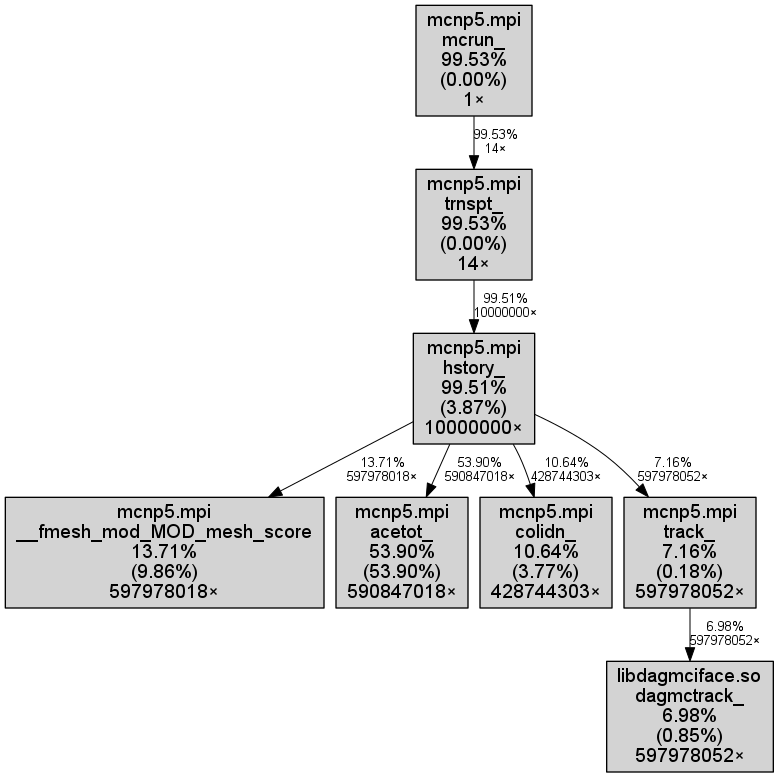
\includegraphics[scale=0.45]{emdag_fng_cg_fine6.png}
  \caption{Callgraph of the EmDAG run on the FNG model for 1E7 histories. (Processes taking $>=$6\% of the runtime are filtered in order to siplify the callgraph.}
  \label{emdag-fng-coarse}  
\end{figure}
\newpage


While the performance of EmDAG greatly surpases that of DAGMC, it does not come as close to the performance of native MCNP as it did in the more simple transport test models. Upon visually inspecting the faceted FNG model, it was seen to contain many high valence regions. As an artifact of the variance reduction used in the intended analysis of this model, many planes were inserted in the model in order to break up large cells with highly varying particle intensities. Where these planes intersect the cylindrical volumes of the model, many high valence regions result as can be seen in Figure \ref{fng-faceted-models}. As a result it became a curiousity as to whether or not the high valence regions were being handled better by EmDAG than they were by DAGMC. In order to test this, the same programs used to do the high valence vertex study were built using EmDAG and the parameter study of the relative high valence area and valency was performed. The results in Figure \ref{emdaghvstudy} show that EmDAG also struggles with these high valence regions. In the worst scenario there is a degradation by two orders of magnitude compared to the best case scenario which is similar to what seen in the unmodified MOAB ray tracer. Additionally, it shows degraded performance in the same way that DAGMC was initally expected to falter - with increasing high valence area and valency. This is likely due to the nature of the heuristics used by Embree to construct its acceleration datastuctures.  Unlike MOAB, however, the BVH building parameters are not as openly available via Embree's interface.There is, however, an option to reduce the size of the high valence regions in the mode within the faceting algorithm by definig a length tolerance.

\begin{figure}[H]
  \small
  \begin{center}
    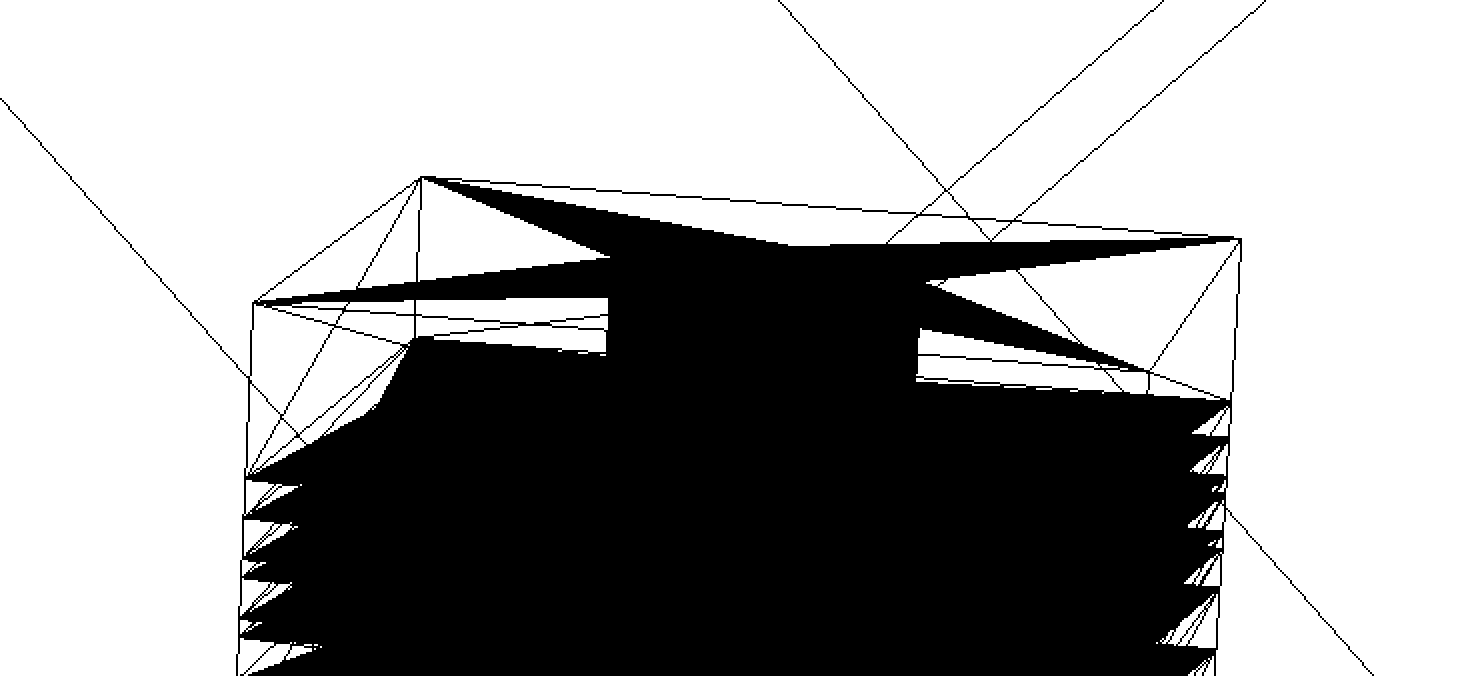
\includegraphics[scale=0.3, trim = 200 0 100 0]{fng_facet_tol.png}
    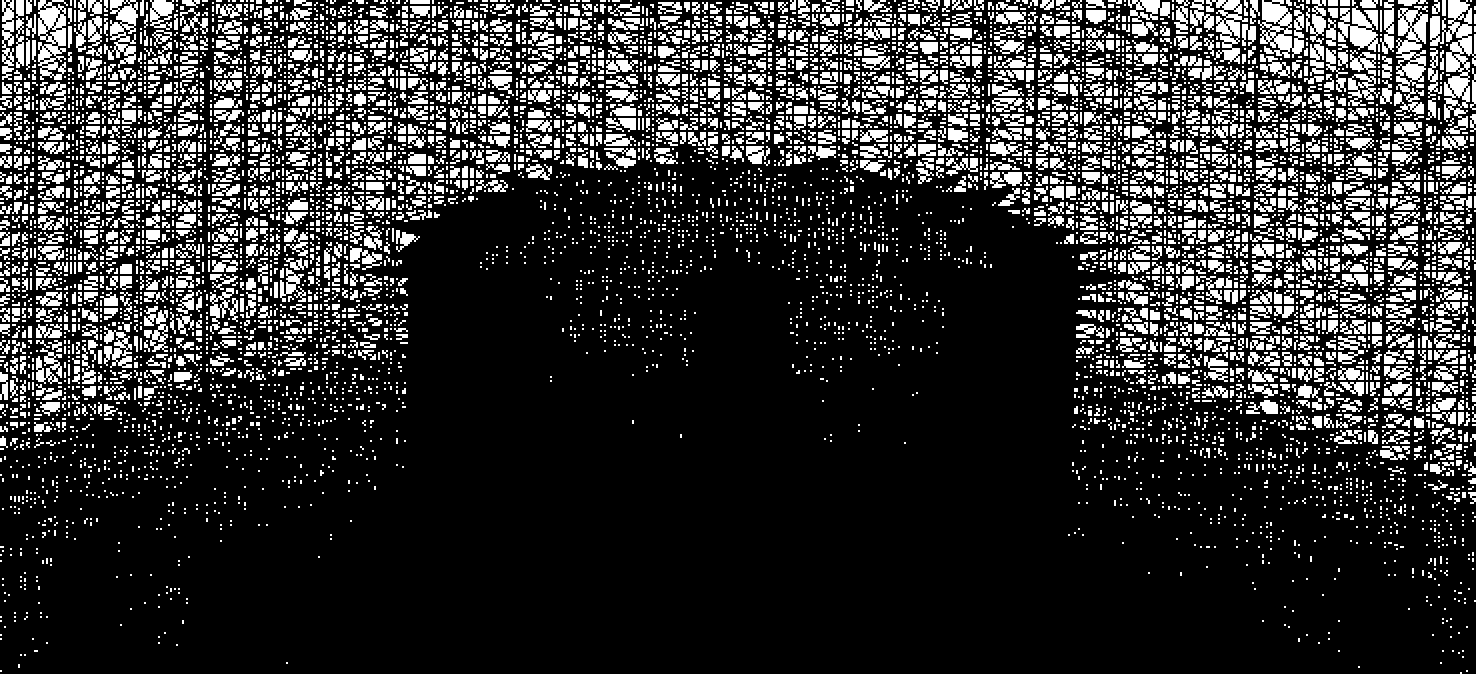
\includegraphics[scale=0.25]{fng_len_tol.png}
    \caption{The FNG faceted model without (left) and with (right) the length tolerance applied.}
    \label{fng-faceted-models}
  \end{center}
\end{figure}

The length tolerance is a maximum length for any facet edge returned by the CAD engine's faceting algorithm. Providing this value to the preprocessing tool comes at the cost of many more triangles than when supplying only a faceting tolerance. The difference in facet structure between these models can be seen in Figure \ref{fng-faceted-models}.

By generating a faceted model using the combination of the length and faceting tolerances it was hoped that there would be a marked increase in performance using the EmDAG system and the performance did indeed improve by ~15\%. Due to the increased number of overall triangles on these planar surfaces, there may be competing forces at play. As the length tolerance is reduced, the high valence areas will also be reduced, but the overall number of triangles will increase - resulting in inherently deeper BVH and longer traversals. Conversely, as the length tolerance is increased, the high valence region areas are increased, but the number of redundant triangles is reduced improving the average BVH traversal time enough compensate for a few more rays entering high valence regions. This observation leads to the idea that length tolerance of the FNG model could then be optimized. This optimization study, while interesting, will vary model to model and the results will be complex in nature, depending on the underlying geometry and geometry adjacent to those regions, etc. In light of the high valence study results showing that BVH building parameters can be altered to improve performance and accomodate these high valence regions, it seems that a better solution is to follow that path over alteration of the mesh globally in the model.

%Nonetheless, while it may be possible to alter the building parameters of Embree as was done with MOAB, but an interface for this does not currently exist within the Embree API and would likely require large alterations to code to allow access such as that. Given these truths, in order to determine how close the current EmDAG system could come to native MCNP performance on the FNG model with the tools available a number of length tolerances were tried when faceting the FNG model.  

\begin{figure}[H]
  \begin{center}
    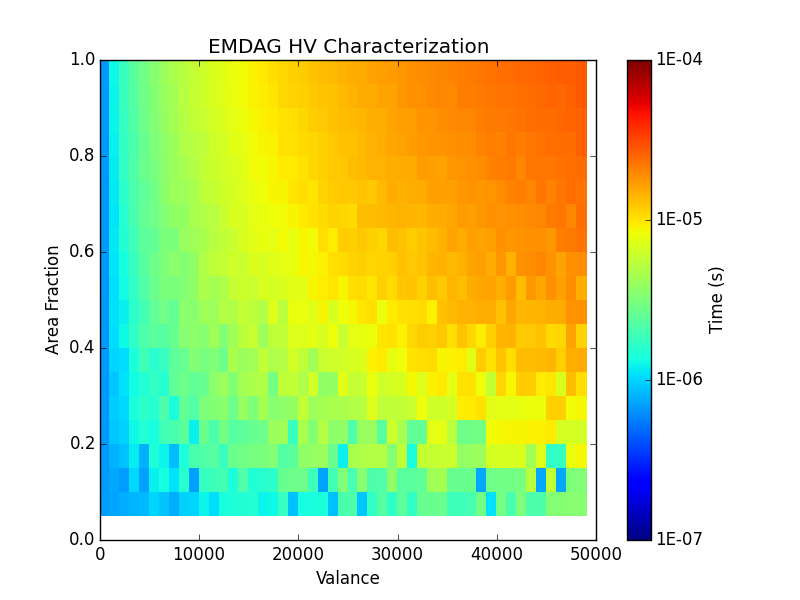
\includegraphics[scale=0.55]{hv_emdag.png}
    \caption{High valance study results using EmDAG.}
    \label{emdaghvstudy}
  \end{center}
\end{figure}


\subsubsection{Limitations of the EmDAG system}%%Status:In Progress%%

While the implementation of Embree in DAGMC showed a vast improvement in performance relative to DAGMC's current implementation, several problems were encountered during the process. This is not surprising when repurposing a ray tracing kernal for an unintended application.

One of these problems is the presence of lost particles in a watertight model. The FNG model EmDAG was tested on is a fully sealed model via the make\_watertight algorithm. A fully sealed model is one in which every volume is topologically sealed such that there are no gaps between surfaces or adjacent volumes. As a result, DAGMC is able to robustly track particles through such a model with no lost particles. While the lost particle rate for the EmDAG FNG test relatively low, they in theory should not occur at all as was shown by the DAGMC runs. After a considerable amount of investigation as to the nature of these lost particles, their cause was determined to be systematic problem not encountered in the nested volume cases due to the simple nature of their geometric topology.

In the DAGMC workflow, a required step for a watertight model is to imprint and merge the surfaces within the CAD system before faceting the model. Imprinting is the process by which Trelis, the CAD software used to generate DAGMC models, makes surfaces and curves that are coincident in space be fully coincident. This process is accomplished by splitting entities into their coincident and non-coincident parts. The merging process then topologically combines these coincident parts into single entities such that the single entities are topologically adjacent to all entities bounding the original set of entities that were merged into one. The result of these steps is non-manifold model with surfaces shared between neighboring volumes \cite{Smith_2011}.

This imprinting and merging of surfaces allows only one representation of each topological entity to be created upon faceting the model. By using the faceted curves of the model as a reference for where surfaces meet in space, the triangles of a surface are then made to meet at those curves in a topologically watertight manner via the \textit{make\_watertight} algorithm. Topologically watertight in reference to triangle facets refers to shared connectivity between surfaces which is distinctly different than watertight by proximity. This topological watertightness of mesh refers to the fact that triangle surfaces meshes have connectivity at their interface which share vertex handles inside of the MOAB database. These vertex handles will then point to the \textbf{exact same floating point representation} of the vertices no matter which of the surfaces is being queried. In this way particles are not lost through gaps in surfaces and firing a ray from the logcal position inside a volume should always result in a triangle intersection. This is not the case however when using EmDAG. Particles were somehow being lost in the transport process.

\begin{figure}[H]
  \centering
  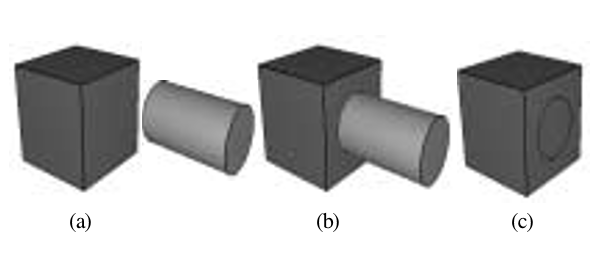
\includegraphics[scale=0.5]{imprint_ex.png}
  \caption{Example of two adjacent volumes being imprinted and merged. a) Two volumes, a cube and cylinder are created. b) The cylinder end face is moved such that it is coincident with one of the faces of the cube. c) The imprint operation is performed and the cylinder curve is imprinted onto the cube (cylinder was removed for visibility of imprinted curve). Adapted from \cite{White_2002}.}
  \label{imprint_ex}
\end{figure}

Some detailed debugging of this problem revealed that this occurs in a systematic fashion within the FNG model at intersections of 3 or more volumes. The secnario is that a particle moves into the intersection between two surfaces. When this occurs, an intersection with either surface connected to that interface is a valid hit so long as the surface is part of the volume the particle is current positioned within. The particle will then logically move into the volume on the other side of the hit surface. EmDAG handles most of these cases well but for the case in which a particle will have a zero track length inside one of the volumes. A zero track length in this case meaning that the particles trajectory is such that it will only glance a volume without having any appreciable track length inside of it. In this case, the EmDAG system may be unable to find a hit whereas DAGMC's tracking is robust enough to find the triangle intersection on this volume and move on.

\begin{figure}[h!]
  \begin{centering}
    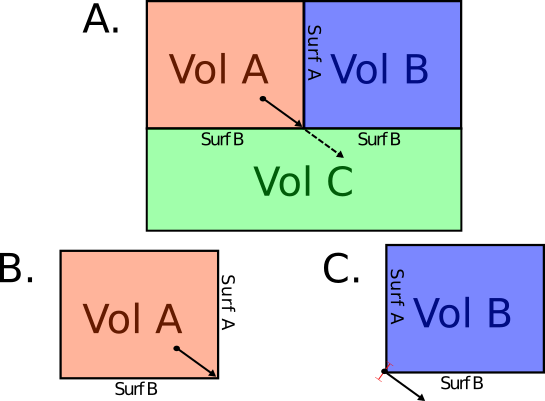
\includegraphics[scale=0.7]{emdag_lost.png}
    \caption{\textbf{A)} The initial scenario of the lost particle. The particle's trajectory is such that it intersects with the boundary between surfaces A and B. The correct continuation of the particle into volume C is depicted as a dashed line. \textbf{B)} An intersection with surface A is found though either surface A or B are equally valid. The particles position is then updated to its intersection with the boundary of surfaces A and B. The particle then logically moves into volume B. \textbf{C)} Upon establishment of the particle in volume B the Monte Carlo code requests the distance to next surface intersection. The particles position and direction are converted from double to single precision. The small change in the particle's position places it outside of volume B and the trajectory is such that an intersection is not found. At this point the particle is considered lost.}
    \label{emdag-lost-particles}
  \end{centering}
  \end{figure}

By isolating this particle's history and producing the particle history with locations precise enough to detect the descrepancies between EmDAG and DAGMC, it was found that the position of the particle in EmDAG was numerically too far outside of a volume to produce the correct triangle hit in either EmDAG or DAGMC's ray fire systems. The cause of this descrepancy is believed to have to do with the necessary conversion between double and sinble floating point precision in the EmDAG system.

As mentioned before, EmDAG uses single floating point representation in its ray tracing kernel while DAGMC uses a double precision representation of the geometry and particle information as does MCNP. In order to accomodate Embree's representation, properties of the particle location and direction are converted to single precision for ray tracing queries in Embree and back to double precision when in DAGMC. When changing the floating point representation, rounding rules based on the computing environment are used to determine the new representation according to IEEE standards for conversion between precision levels \cite{IEEE_STD_2008}. These changes in the particle's location and direction are small, but in the scenario described above it seems that the particle location and/or direction are altered enough throughout the course of its history to cause a failed ray intersection - resulting in a lost particle.


In Brandon Smith's thesis, ``Robust Particle Tracking and Advanced Geometry for Monte Carlo Radiation Transport'' \cite{Smith_2011} there is a detailed description of the different pathologies encountered in tracking particles through a surface mesh representation of a geometric model. Briefly mentioned in this chapter is the possibility of a lost particle due to numerical error in the particle's position perpindicular to the particle's trajectory. Lost particles caused by this pathology are not covered however as the double floating point representation does not allow the particle position to change enough for this case to occur in practice. In EmDAG, however, this particular pathology is now vulnerable due to the constant conversion from single to double precision values between DAGMC and Embree. In order to avoid this problem moving forward, any improvements to DAGMC's ray tracing kernel for particle tracking will need to maintain use of double precision representations for mesh elements for robust coupling of numerical and logical particle positions and directions.

\section{Research Proposal}%%Status:In Progress%%
\label{research_proposal}

This chapter outlines a short summary of the motivation for this work, and outlines the work to be done supported by previous work of the author.

The performance of CAD-based transport is a concern moving forward in the area of Monte Carlo radiation transport, particularly in relatively new areas such as high-energy physics devices or fusion energy systems. In comparison to well-established CSG modeling of geometries, the performance is several times worse as down in Section \ref{perf_benchmark}. DAGMC is a robust tool for tracking particles through surface meshes of CAD models, but can be made more efficient using the various approaches outlined below. This proposal will outline three different approaches for improving CAD-based transport performance in the DAGMC toolkit.

\subsection{SIMD-Enabled Acceleration Data Structure}

As described in Section \ref{emdag}, a SIMD-enabled ray tracing kernal, Embree, has already been applied within the DAGMC framework with great success. Unfortunately some aspects of DAGMC's robustness were lost due to a fundamental difference in the precision used to store geometric primitives and intersect rays. It is believed that this problem can be remedied in a straightforward manner by altering these datatypes from single to double floating point precision to match those of the underlying physics codes DAGMC supports and adjusting the underlying algorithms accordingly. A substantial reduction in performance due to this change in floating point calculations is not expected however as the construction of the underlying hierarchy used to isolate triangles for intersection can remain in single precision if built appropriately. Others have noted such a benefit from reduced-precision bounding volumes in the past as well\cite{Mahovsky_2005}.

%Estimation of performance change here%

%% \begin{figure}
%%   \begin{equation}
%%     \sum_{}^{N_r}T_T + I\sum_{}^{N_r} P_{n}
%%   \end{equation}
%%   \caption{A theoretical estimation of the performance reduction in Embree when using geometric primitives with double precision.}
%%   \label{perf_estimate}
%% \end{figure}


Two options to accomplish the above goal of applying SIMD-enabled ray tracing robustly within DAGMC will be explored and the more advantageous one selected for implementation. The first is to alter Embree to meet the requirements of higher precision primitives, expanded single precision bounding boxes to contain all double precision entities, and link this updated version to the MOAB primitives as was done in previous work. A member of the Intel development team has indicated that this process may already be underway. An alternative approach is to design a kernal with many of the features that exist in Embree but that couples more cleanly with DAGMC's underlying mesh database, MOAB. Embree is an excellent kernel, but its focus may be too broad for the purposes of DAGMC. Omitting some of the existing features within Embree such as dynamic surface representation and support for hair geometries \cite{Woop_2014} will allow for a more simple design and implementation for future researchers. MOAB's database oriented design does not easily support such a kernel directly, but its ability to store data in a contiguous manner and provide direct access to that data is a unique feature that would allow it to interact directly with a SIMD-enabled ray tracing kernel that is more catered toward the current needs of the scientific community.

The new ray tracing kernel will be applied to the performance benchmarking models used in Section \ref{perf_benchmark} to demonstrate its capability to maintain DAGMC's current robustness but with significantly improved performance. A reduction in the memory footprint of DAGMC should also be seen due to the combined effects of reduced-precision bounding boxes and a shallow hierarchy design.

\subsection{Special Case Allowance in BVH Building}

Historically, DAGMC's performance has suffered due to high-valance mesh features. In Section \ref{hv_study} of this work it was established that the resulting performance degredation came from difficulties in building an effective hierarchy in mesh regions containing this feature and that this problem could be remedied with a small alteration to MOAB's BVH building algorithm. Furthermore, it was established that this mesh feature was problematic not only for DAGMC's building algorithm but also for Embree's which uses a different heuristic to build its BVH datastructure. Given this information, it is proposed that pathological mesh features such as high-valence regions be given special attention when building a BVH despite the extra time this may take for models with many of these regions.

In Monte Carlo radiation transport, a significantly higher number of ray queries are made than in rendering. In order to obtain a statistically valid anser to the problem at hand, the number of primary rays is generally an order of magnitude higher than that of a rendering problem in which a fixed number of primary rays are fired per pixel in the desired view (see Figure \ref{render_ray_estimate}). Additionally, the number of secondary rays is much higher in radiation transport than in rendering due to the nature of the underlying physics and variance reduction techniques employed. In either ray tracing application, the time to solution can be roughly described by the time needed to construct the necesary acceleration structures and satisfy the ray queries.

\begin{figure}[H]
  \centering
  Rendering: \\
  $ (8\, rays\, per\, pixel)\, \times (1024 \times 1080\, pixels) = 16.6 \times 10^6 $ primary rays \\
  Monte Carlo: \\
  ITER analysis standard number of histories = $ 1 \times 10^9 $ primary rays
  \caption{An  estimation of the number of ray queries in a typical rendering vs. in common ITER analysis performed using DAGMC. The number of pixels per ray was determined by common practice in rendering.}
  \label{render_ray_estimate}
\end{figure}

Figure \ref{tts_est} provides an esimate of the time to solution for a ray tracing based process in a similar manner to which Hurley performs this analysis in \cite{Hurley_2002}. The time it takes to perform the ray tracing queries is partially dependent upon the quality of the acceleration structure being built. The better the quality of these structures, the faster the ray queries will be satisfied and the solution reached. The quality of the accceleration datastructure is also dependent on the amount of time spent in building the datastructures. Presumably the more time spent building the datastructure, the better its quality. By establishing this dependence of total ray traversal time on the time spent building acceleration datastructures, the result is an optimization of the time spent building the right quality of acceleration datastructures for the lowest time to solution. 

Typically, rendering tools focus on building a generalized data structure with respect to the mesh its operating on without consideration of the more subtle features of the mesh and how the datastructure's quality might be improved. This is commonly because the time spent in improving the quality of the datastructure is overly costly compared to the total amount of time saved when performing the ray queries. In the scenario of Monte Carlo radiation transport, the saved time in performing necessary ray queries may become significant, making the extra time spent in building the acceleration datastructures to increase their quality becomes favorable. The trade offs of these costs/savings are difficult to quantify in that they vary greatly model to model - as is the case for most a priori ray tracing performance evaluations. However, the severe degredation in ray fire performance due to mesh features produced by triangulation algorithm on which DAGMC relies leads one to believe that time spent adapting to such mesh features is worthwhile.

\begin{figure}[H]
  \centering
  \begin{align*}
    tts =\, & C + T_{B} + \sum_{}^{N_{r}} T_{T} \\
    tts =\, & C + T_{B} + \sum_{}^{N_{r}} T_{T}(q,\ldots) \\
    q(T_{B}) & \rightarrow T_{T}(T_{B}) \rightarrow T_{T} \propto \frac{1}{{T_{B}}^{x}} \, (where \, x \geq 0) \\
    tts =\, & C + T_{B} + \sum_{}^{N_{r}} T_{T}(T_{B},\ldots) \\
    tts \, - & time\, to\, solution \\
    C \, - & cost\, of\, operations \, not \, reliant \, on \, ray \, tracing \\
    T_{B} \, - & acceleration\, datastructure\, build\, time \\
    T_{T} \, - & average\, traversal\, time \\
    N_{r} \, - & ray\, queries \, required\, for\, solution \\
    q \, - & acceleration\, datastructure\, quality \\
  \end{align*}
  \caption{General equation for the time to solution of a ray tracing based process.}
  \label{tts_est}
\end{figure}

While one could imagine a process in which high-valence regions could be detected and isolated in a global manner for the entire surface mesh and parameters adjusted when those regions are encountered, this process could be very computationally expensive with little reward if no high-valence regions exist or if they are inconsquential during problem execution. Conveniently, the building algorithms tend to isolate such regions naturally as poorly formed leaf nodes. If the branch of the hierarchy terminates at a poorly formed leaf, detection of a high-valence region can be performed on this portion of the mesh contained by the leaf and a specialized building algorithm could be applied should one be found. This process may occur after the hierarchies' normal build is complete via tree analysis or the poorly formed leaves may be handled as they are encountered during the intial build. Whichever implementation is used, it will be applied in such a way that it is easily extended to other such pathologies in CAD-based surface meshes as they are encountered in the future.

This extended building scheme will be implemented within the ray tracing kernel mentioned above and applied to the high-valence study model as well as transport problems known to cantain high-valence regions to demonstrate is ability to provide an improvement in performance for models produced by the faceting algorithms used in DAGMC's recommended workflow.

\subsection{Signed Distance Field Preconditioner}

A signed distance field defined over the domain of a volume will be applied as a pre-conditioning tool for DAGMC's ray fire process to avoid full reliance on ray tracing when possible.

As described in the introduction of this work, a particle's current location along with the intended next physical interaction location is provided to DAGMC by the physics code it is interfacing with. DAGMC is then expected to return confirmation that the particle has not crossed a surface of the current volume in which the particle resides by returning a value larger than the distance to the physical interaction location or to return the distance to the surface intersection as well as which surface it has crossed. It is proposed that a preconditioner be added to DAGMC in order to avoid unnecessary ray tracing calls for locations relatively far from surface boundaries via methods associated with implicit surfaces. Section \ref{implicit_surfaces} of this work discusses the used of implicit surfaces and their derived signed distance fields in the applications of vizualization and rendering. Specifically, a signed distance field stored on a structured cartesian mesh over the volumes of a model will be applied to provide $O(1)$ access to information for point containment and particle tracking queries via interpolation for points of interest within the volume domain.

\subsubsection{Preconditioning of Point Containment Queries}

The use of a signed distance field for point containment queries is rather straightforward. First the point of interest will be determined to be inside or outside of the volume's bounding box as is currently done in DAGMC. If the point is determined to be inside of the bounding box, an interpolation of the point's signed distance value will be performed with the sign of the value indicating the point's containment. It is important to recognize that any sampling and interpolation of a function will come with associated error. This will be addressed later in this section, but for now it will suffice to say that if the magnitude of the value is smaller than an appropriately determined error tolerance for the signed distance field, then the point containment process will defer to the previously relied upon ray tracing process as before.

\subsubsection{Preconditioning of Nearest Intersection Queries}

Nearest surface intersection's along a particle trajectory will be preconditioned using the interpolated signed distance values of both the current particle location and the interaction location provided by the physics code. The summation of these two values are a representation of the minimal free space between them and a surface intersection. This value can then be compared to the distance from the particle's location to the interaction location to determine if a ray fire is necessary. As shown in Figure \ref{preconditioner_ex}, if the combined minimal distance from the two signed distance values is greater than the distance to the next interaction location then the ray fire can be skipped. If not, then this indicates that the particle may intersect a surface before reaching the interaction location and a ray fire should be performed to confirm this. The final situation presented in Figure \ref{preconditioner_ex} is one in which the distance is accounted for but due to the error associated with the interpolation process the logical result is ambiguous and a ray fire is needed to robustly determine the nearest intersection distance. 

\begin{figure}[H]
  \centering
  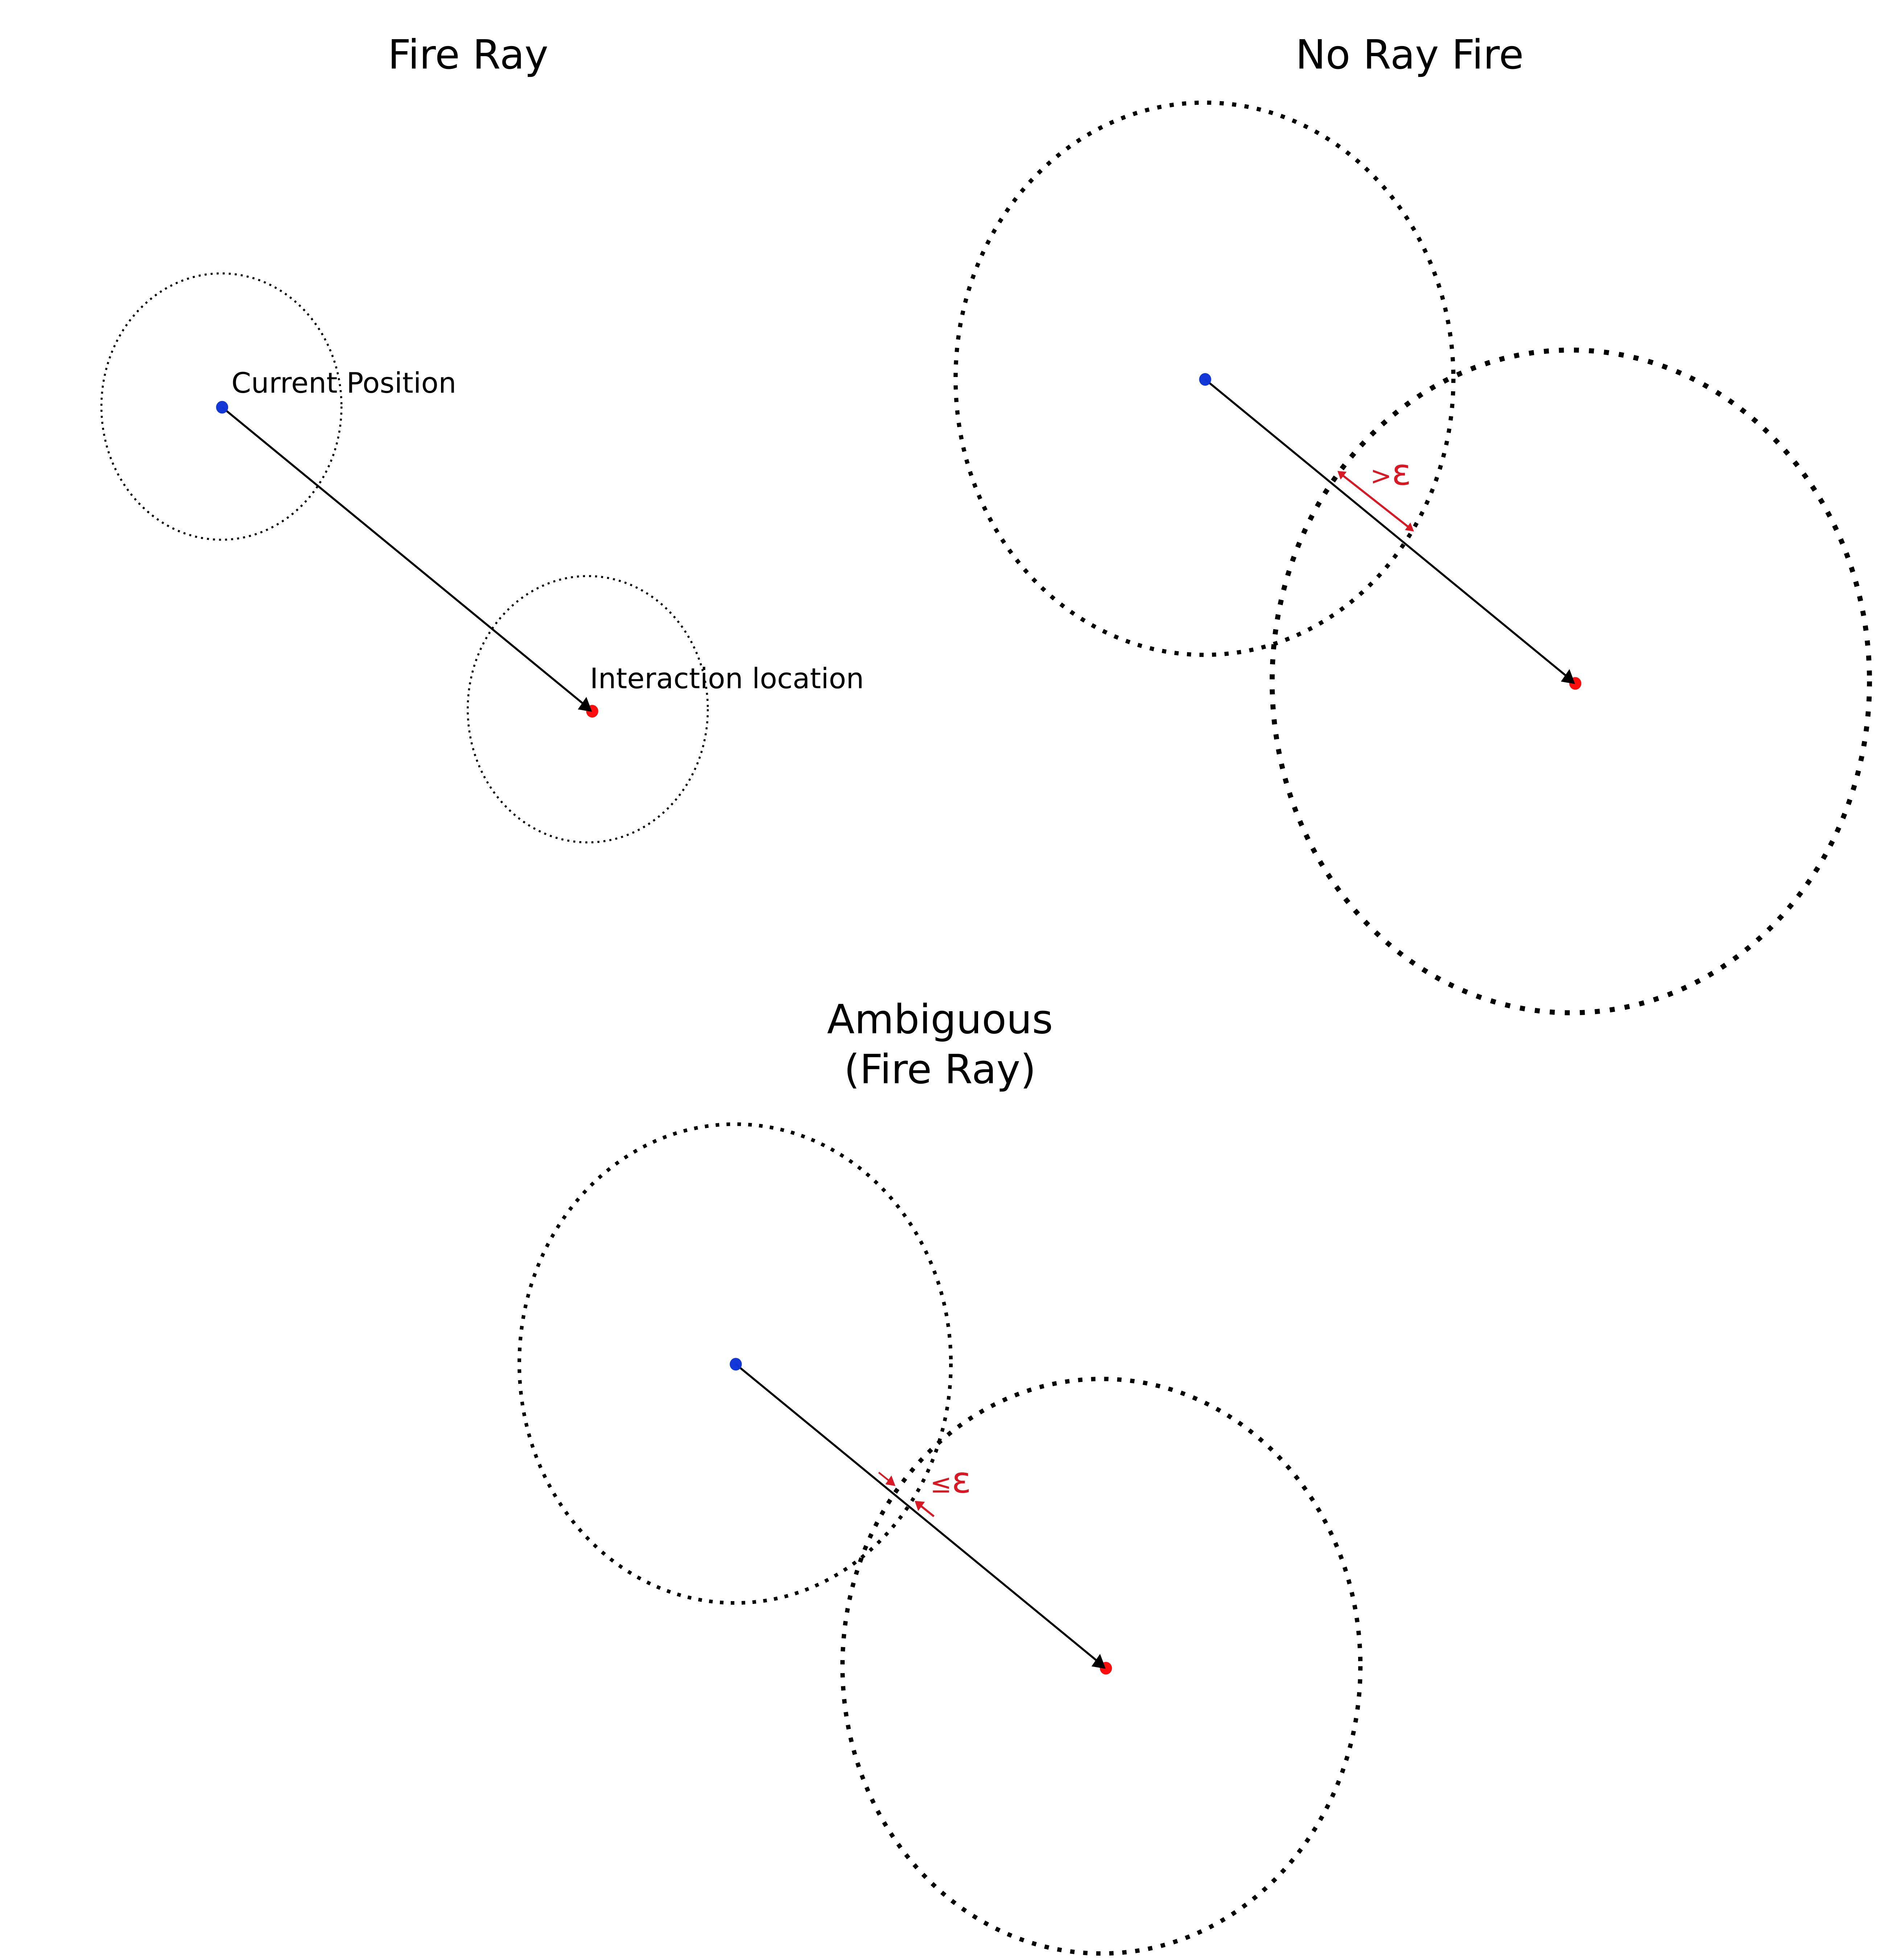
\includegraphics[trim = 50 0 0 0 , scale=0.6]{preconditioner_ex.png}
  \caption{Example of how signed distance values at the beginning and end of a ray can be used to avoid un-nessecary ray queries. a) The ray fire process can be avoided as it has been definitively shown that there is no interface intersection. b) A ray fire must be performed as it is possible there is a surface intersection between the two points of interest. c) The signed distance values indicate that a ray fire can be avoided but not definitevly when accounting for error - a ray fire must be executed.}
  \label{preconditioner_ex}
\end{figure}

\newpage


 \subsubsection{Preconditioner Datastructure}

 As mentioned earlier in this section, it is envisioned that the signed distance values for each mesh node can be stored in a structured mesh framework with equal mesh intervals in each dimension for simplicity. Because this datastructure will initially be applied to all volumes in a model, its memory footprint will be managed by only storing a corner of the mesh, the step size of the mesh, the number of intervals in each dimension, and the signed distance values in a flat array. A tri-linear interpolation for any point within the mesh bounds can then be performed using data values gathered from the array via direct lookup. This will be done finding surrounding mesh node indices provided by the number of intervals in each dimension using the mesh corner to the point of interest.
 
While implicit surfaces provide a natural way to populate such a mesh with signed distance values and can be generated from triangle mesh structures like the ones used in DAGMC, this can also be accomplished using BVH algorithms for finding the nearest triangle intersection in any direction without added support for implicit surface generation and handling. Using the same structure to retrieve signed distance values is also important for self-consistency between the preconditioner and ray tracing kernel. The imporantance of this has been experienced before \cite{Smith_2011}.

\subsubsection{Interpolation Error Estimation}

While mentioned breifly in the sections on application of the preconditioner during transport, signed distance values interpolated from the mesh will come with some associated error. A conservative estimate of this error is a critical component for robustness during transport of particles. The biggest concern being that empty space is incorrectly declared between the particle location and the next event location in which case the particle's numerical and logical position will become inconsistent.

The typical error associated with an interpolcation of this type is $O(h^3)$ where $h$ is the step size of the mesh. As seen in Equation \ref{interpolation_err_2d}, the error associated with a two dimensional bilinear interpolation is also dependent upon the curvature of the surface. While for the majority of cases one can expect that the mesh error will be dominant in this formula, the fiedlity of simulation results is put at risk if this is not well-understood. A stringent set of unit test cases will be developed to ensure robust use of the preconditioner as well as comparison to previous DAGMC-based simulations which rely entirely on the ray tracing process to verify results produced using this method.

\begin{figure}[H]
  \begin{equation}
    \epsilon = \frac{1}{2} \Delta x (h-\Delta x) \frac{\partial^2 u}{\partial x^2} + \frac{1}{2} \Delta y (h-\Delta y)  \frac{\partial^2 u}{\partial y^2}
  \end{equation}
  \begin{align*}
    h - & \, mesh\, interval\, size \\
    \Delta x - & \, x\, distance\, to\, interpolation\, point\, from\, data\, point \\
    \Delta y - & \, y\, distance\, to\, interpolation\, point\, from\, data\, point \\
    u(x,y) - &\, sampled\, function\, on\, mesh \\
    \epsilon - & \, error \\
  \end{align*}
  \caption{Taylor expansion of 2D interpolation equation as an estimate for the error of a function sampled onto a structured cartesian mesh.}
  \label{interpolation_err_2d}
\end{figure}

There are several cases in Monte Carlo for which the use of a ray tracing preconditioner will be wasteful. Obvious cases include low density volumes, void volumes, or very small volumes. These cases can be further generalized as volumes for which the average mean free path is large relative to its size. Meaning that particles are more likely to cross a surface than not. This observation leads to the question of how to quantify such a characteristic for use in discerning when the application of this preconditioner is effective. For the purpose of this research, the signed distance preconditioner will be applied indescriminantely for each volume with the exception of void volumes.

This method is expected to be particularly effective in transport simulation of charged particles who's curved paths are often modeled as a series of small segments, each of which requires next intersection confirmation throughout the particle's history. This hypothesis will be tested by applying the preconditioner in Flu-DAG, a version of DAGMC coupled with Fluka\cite{Bohlen_2014}, which has the capability for such charged particle transport.

\subsection{Summary}

Three areas of improvement have been identified as valuable additions to the DAGMC radiation transport toolkit. A SIMD-enabled ray tracing kernel which takes advantage of MOAB's direct access and contiguous memory capabilities will improve the performance of DAGMC's current tracking algorithm while maintaining the rich mesh-based representation with underlying topological attributes. From previously gathered data in Chapter \ref{experiments_and_data} this improvement alone is expected to improve DAGMC's performance many times over, achieving speeds on the order of native geometry handling in native Monte Carlo Codes.

A specialized extension of the bounding volume hierarchy builder has been proposed to accomodate mesh features which result in poorly formed acceleration data structures for the standard heuristics or parameters used in their construction. These poorly formed leaf nodes containing high valence regions have been shown to be highly obstructive to the ray tracing algorithms even for relatively small features and a remedy for this solution has been demonstrated which returns the datastructures to their expected performance values. While high valence regions are the only currently known mesh feature which different building algorithms struggle to process, a workflow will be left behind in which similiar problematic features can be isolated, characterized, and accomodated in the future.

For particles commonly interacting away from the boundary of volumes, the ray tracing process may be overly precise and expensive for a simple determination of whether or not the particle crosses a surface. The implementation of a rudimentary preconditioner based on techniques used in implicit surface rendering has been proposed. This preconditioner will store a signed distance field populated by the ray tracing kernel to provide an $O(1)$ check for unambiguous situations in which both the particle and its next intended location are far enough from the boundary of the volume that a ray fire process is un-needed, allowing the particle's transport to continue unimpeded. In this way the ray tracing process is reserved for situations in which its precise answer is necessary, preserving the capability for robust transport in DAGMC.

Each of these areas provide a benefit to DAGMC's performance on their own, but it is hoped that the combined effects of these improvements will be most pronounced when used together for greatly improved perforamnce using CAD-based models. For example, the use of a pre-conditioner can help to avoid ray fires, but there will always be situations in which a ray query is necessary to provide an unambiguous answer about the particle's next step in transport. The improvements to the underlying ray traversals via SIMD and a specialized building algorithm for handling of high-valance regions will also result in improved performance when these situations are encountered. At the same time it can also be stated that the application of any of these methods individually will also improve the performance of DAGMC to some degree.

\subsection{Contributions}

This section concisely states the specific contributions of the three areas described in the research proposal.

\subsubsection{SIMD-Enabled Acceleration Data Structure}

SIMD traversal of BVH's has been shown to greatly improve the performance of CAD-based radiation transport by DAGMC's use of Embree, but cannot be made robust using this kernel as it exists now. A new data structure is proposed which will maintain much of the performance improvement seen in EmDAG by building and traversing single-precision bounding volumes around double precision primitives. It is proposed that utilization of this mixed-precision system will allow for a ray tracing kernel with performance rivaling those of native geometry representations (CSG) on common CPU architectures while meeting requirements of DAGMC's particle tracking algorithm.

\subsubsection{Special Case Allowance in BVH Building}

High valence regions studied in this work are common features seen in surface faceting algorithms. The impact of these features can be mitigated by applying a maximum facet edge length tolerance to reduce their size, but this can greatly increase the overall memory of a model. A method for maintaining performance by altering median splitting parameters has been demonstrated. Applying a similar building method or by modifying the SAH method in production models, ray tracing performance can be maintained without additional memory cost of extra primitives or mesh manipulation. This will also involve the creation of a generalized building process in which poorly formed leaf nodes of the hierarchy are revisited and re-evaluated for mesh problematic features if they are detected. This data structure optimization is of particular interest for the application of radiation transport in comparison to rendering applications for which the extra time spent rebuilding leaf nodes may be a more significant portion of the total time to solution.

\subsubsection{Signed Distance Field Preconditioner}

A signed distance field allows DAGMC to rely on an O(1) process when tracking particles far from surface interfaces, falling back onto the robust O(log(N)) ray tracing process only when necessary. This data structure has been used for directly rendering surfaces, but never as a preconditioning tool for particle tracking before. Because this data structure will be applied to a static mesh and only needs to be populated once, DAGMC's ray tracing kernel could be used to populate the data structure without the need to generate an implicit surface representation. Also of interest is the possibility of coupled acceleration data structures in which information from the signed distance field structure can enhance the ray tracing kernel's performance during simulation.


%% In order to make CAD-based Monte Carlo competitive with native codes it is clear that geometry queries must be satisfied much more quickly than the ray tracing kernel in DAGMC can currently provide. Investigation into the shortcomings of the DAGMC ray tracing process have revealed various opportunities for improvement. One in implementation and the other in application.

%% One aspect of these improvements rely on removing the ray tracing kernel from implementation restrictions associated with it being written in the context of a database system and being confined to construction of those database elements. Separation of the kernel allows for a simplified and streamlined system which may be allowed to take advantage of any set of optimizations available in the world of computing. The coupling of DAGMC to Embree provides good evidence of the combination of these assertions. Embree, being an entirely standalone software tool, is inherently free of the databse context in which MOAB's ray tracing tools exist. Additionally, Embree takes advantage of hardware acceleration techniques in the form of single instruction multiple data (SIMD) avilable on most machines.

%% The Embree ray tracing kernel while very powerful is still oriented toward a rendering application in which a fixed number of primary rays is required to resolve each pixel's color with some secondary rays resulting as dictated by the physics of the model. Similarly, the oriented bounding box (OBB) hierarchy is adapted from a method initially used for interference detection of objects in virtual space. While the application of ray tracing for the purpose of rendering is perhaps closer to the desired application of ray tracing in Monte Carlo than that of interference detection, subtle differences in these applications exist. In optimization, subtleties can greatly impact performance if approached appropriately. One such example in the application of rendering is the recent movement toward firing of rays in packets, taking advantage of the coherency in ray paths coming from a single source. This subtlety is not shared in the realm of Monte Carlo for radiation transport an identical starting condition for a particle can result in a very different pathway through the geometry due to the stochastic nature of a high energy particle's interaction within a medium. It is differences like these that cultivate interest in other properties of Monte Carlo radiation transport that may alter one's approach to design of a ray tracing kernel.

%% Time it takes to perform the ray tracing queries is partially dependent upon the quality of the acceleration structure being built. The better the quality of these structures is the faster the ray queries will be satisfied and the solution reached. The quality of the accceleration datastructure is also dependent on the amount of time spent in building the datastructures. Presumably the more time spends building the datastructure, the better its quality. Typically, rendering tools focus on building a generalized data structure with respect to the mesh its operating on without consideration of the more subtle features of the mesh and how the datastructure's quality might be improved. This is commonly because the time spent in improving the quality of the datastructure is overly costly compared to the total amount of time saved when performing the ray queries. In the scenario of Monte Carlo, it has been established that many times the number of rays are being fired in order to obtain the solution several times over. In this case the saved time in performing necessary ray queries may then become significant, and that the extra time spend in building the acceleration datastructure to increase its quality becomes favorable. The trade offs of these costs/savings are difficult to quantify in that (as is the case for most ray tracing performance evaluations) they vary greatly model to model. However, the severe degredation in ray fire times due to mesh features produced by the surface mesh generation algorithm on which DAGMC relies leads one to believe that adapting to such mesh features and any other such features discovered in the future is worthwhile.

%% To address the issues of the implementation context and add mesh adaptive qualities to the BVH build process, a new ray tracing kernel is propsed. This kernel will have components both inside and outside of MOAB. MOAB is currently used to represent DAGMC model topologies as well as their discretized representations. These meshes are generated inside MOAB and as such MOAB has access to alter, manipulate, and query all information about the mesh. It also provides a rich set of mesh manipulation, detection and generation tools. Most importantly, MOAB provides the capability to gaurantee contiguity in memory for both mesh elements and mesh-related data via dense tags. This is a key requirement for many of the efficiencies made available by vectorized operations during traversal of the datastructures. MOAB's unique ability to provide this contiguous data allows one to link its powerful generation, adaptation tools to any set of low-level optimizations available on current CPU architectures. It does not in itself contain the ability to utilize these optimizations within its database oriented system, however. As a result, the traversal component of the ray tracing kernel will need to be implemented outside of MOAB. There are a few viable options for accomplishing this. Currently, a system close to this exists inside EmDAG but under the hood Embree is creating its own BVH. It may be possible to structure a BVH from MOAB and pass it to Embree as the data structure to use for traversal. Problems related to the conversion back and forth from double to single precision would need to be addressed as they currently violate the parameters of DADMC's robust particle tracking algorithm and its possible that the particular pathology resulting in lost particles in the EmDAG system is impossible to resolve. Another option is to develop a traversal module either alongside or separate from MOAB which allows for robust raytracing on a double precision triangle surface mesh. This option gives more control over DAGMC in the future in terms of the ability to study different acceleration datastructures, support of specific vector extensions, and a simpler implementation. Embree is an excellent tool with support for many features such as subdivision surfaces, advanced techniques for representation and tracing of hair geometry, etc. which are related more to rendering than they are to ray tracing of static surfaces meshes. 

%%%%%%%%%%%%%%%%%%%%%%%%%%%%%%%%%%%%%%%%%%%%%%%%%%%%%%
%%%%%%%%%%% EXTRA STUFF TO DRAW FROM %%%%%%%%%%%%%%%%%
%%%%%%%%%%%%%%%%%%%%%%%%%%%%%%%%%%%%%%%%%%%%%%%%%%%%%%
%% In fact, the specific problem of finding the next closest intersection within a virtual model given a point and a direction is commonly encountered in the area of rendering for 3D models.

%%  As a particle is born, the material in which it exists must be determined as it will dictate the underlying physics of its travel through 

%% This process has allowed for successful transport runs of complex models of the International Thermonuclear Experimental Reactor (ITER) for runs upward of 1E8 histories with zero lost particles.\cite{Smith_2011}

%% Naturally following the ability to do these robust calculations on already complex models, increasingly detailed models are becoming of interest. Unfortunately it has been shown that as detail increases, the performace of DAGMC lags more and more in comparison to the native versions of the various Monte Carlo codes it supports (see Table \ref{DAG-MCNP_performance}). It is known that this performance issue is due to the time it takes to return geometric information to Monte Carlo packages from the ray tracing kernel it relies upon. Historically this has been true of applications which rely on ray tracing processes.\cite{Glassner_1989} In agreement with this trend, this work shows that ~85\% of the run time of DAGMC baed transport is spent in the ray tracing kernel. The remainder of this work details an investigation into the shortcomings of DAGMC's ray tracing process as well as various options for improvement. An important part of this investigation is the analysis of ray tracing from the application-specific perspective of its use in Monte Carlo radiation transport.

%% \begin{table}[H]
%%   \centering
%%   \caption{Table comparing the performance of DAG-MCNP to native MCNP for the same modules after translation to a CAD-based surface mesh.}
%%     \label{DAG-MCNP_performance}  
%%   \begin{tabular}{l c c c}
%%     \toprule \\
%%     Model & Native ctme (min) & DAGMC ctme (min) \\
%%     \hline \\
%%     FNG &  5871.92 & 22769.33 \\
%%     ATR &  901.68 & 8627.80 \\
%%     UWNR &  8767.29 & 69429.60 \\
%%     \hline \\
%%   \end{tabular}
%% \end{table}


%% Each of the ray tracing kernels studied later in this work were initially intended for other applications and adapted for use in Monte Carlo. MOAB's Oriented Bounding Box (OBB) hierarcy was initally designed for use as part of an interference detection algorithm\cite{Gottschalk_1996} while Embree (discussed later) is a ray tracing kernel optimized for the purpose of interactively rendering static or dynamic models. Ray tracing in Monte Carlo differs from each of these applications though it is more closely aligned with the process of rendering than interference detection. Even so, Monte Carlo ray tracing differs from rendering in a fundamental way and deserves to be approached uniquely rather than as an adaptation or extension of another purpose. This is true for a few different reasons.

%% In Monte Carlo, a significantly higher number of ray queries are made than in rendering. In order to obtain a statistically valid anser to the problem at hand, the number of primary is generally an order of magnitude higher than that of a rendering problem. The average number of secondary ray queries is even more so. In radiation transport, interactions may occur at any point in space (depending on the virtual material which occupys that space) rather than nearly always at the interface of object. This increased spatial interaction frequency leads to a much larger number of secondary ray queries ($O(100)$)than one might or could see in a rendering process. In either case, the time to solution (render) can be roughly described by the time needed to construct the necesary acceleration structures and satisfy the ray queries. Figures \ref{render_ray_estimate} and \ref{tts_est} provide an esimate of the number of primary rays required for solution and the time to solution for a ray tracing based process, respectively, in a simiarly manner to which Hurley performs this analysis in \cite{Hurley_2002}.

%% \begin{figure}[H]
%%   \centering
%%   \caption{A rough estimation of the number of ray queries in a typical rendering vs. in the FNG model runs. The number of pixels per ray was determined by common practice in rendering.}
%%   \label{render_ray_estimate}
%%   \[ (8\, rays\, per\, pixel)\, x (1024 x 1080\, pixels) = 16.6M \, rays \]
%% \end{figure}


%% Time it takes to perform the ray tracing queries is partially dependent upon the quality of the acceleration structure being built. The better the quality of these structures is the faster the ray queries will be satisfied and the solution reached. The quality of the accceleration datastructure is also dependent on the amount of time spent in building the datastructures. Presumably the more time spends building the datastructure, the better its quality. Typically, rendering tools focus on building a generalized data structure with respect to the mesh its operating on without consideration of the more subtle features of the mesh and how the datastructure's quality might be improved. This is commonly because the time spent in improving the quality of the datastructure is overly costly compared to the total amount of time saved when performing the ray queries. In the scenario of Monte Carlo, it has been established that many times the number of rays are being fired in order to obtain the solution several times over. In this case the saved time in performing necessary ray queries may then become significant, and that the extra time spend in building the acceleration datastructure to increase its quality becomes favorable. The trade offs of these costs/savings are difficult to quantify in that (as is the case for most ray tracing performance evaluations) they vary greatly model to model. However, the severe degredation in ray fire times due to mesh features produced by the surface mesh generation algorithm on which DAGMC relies leads one to believe that adapting to such mesh features and any other such features discovered in the future is worthwhile.

%% \begin{figure}[H]
%%   \centering
%%   \caption{General equation for the time to solution of a ray tracing based process.}
%%   \label{tts_est}
%%   \begin{align*}
%%     tts =\, & C + T_{B} + \sum_{}^{N_{r}} T_{T} \\
%%     tts =\, & C + T_{B} + \sum_{}^{N_{r}} T_{T}(q,\ldots) \\
%%     q(T_{B}) & \rightarrow T_{T}(T_{B}) \rightarrow T_{T} \propto \frac{1}{{T_{B}}^{x}} \rightarrow x \geq 0 \\
%%     tts =\, & C + T_{B} + \sum_{}^{N_{r}} T_{T}(T_{B},\ldots) \\
%%     tts - & time\, to\, solution \\
%%     C - & cost\, of\, other\, operations \\
%%     T_{B} - & acceleration\, datastructure\, build\, time \\
%%     T_{T} - & average\, traversal\, time \\
%%     N_{r} - & rays\, required\, for\, solution \\
%%     q - & acceleration\, datastructure\, quality \\
%%   \end{align*}
%% \end{figure}

%% Additionally, the way in which rays traverse a model limits the number of possible triangles for a given ray query to the triangles used to form the current volume (cell) in which the particle resides. As a result, trees are created on a per-volume basis whereas in rendering rays are allowed to hit any object in the virtual space. This difference in perspective a manifestation of the underlying physics between the two applications. Most interactions of influence occur inside virtual objects of non-negligible density rather than in the relatively empty space between them. In rendering, most of the interesting interactions affecting the blurring of objects, shadowing, etc. occur in this void or air-filled space between objects.

%% Many ray tracing datastructures, heuristics, and other techniques are explored as part of a review of ray tracing's current state. This is followed by an analysis of DAMC's performance limitations as well as the investigation of known problem-specific difficulties encountered by ray tracing kernels as a result of the process used to generated surface meshes in the DAGMC workflow. Finally a plan is laid out to create a Monte Carlo oriented ray tracing kernel which couples the existing functionality of current tools such as MOAB with some of the more powerful ray tracing techniques currently available and seeks to take advantage of more subtle optimizations specific to its purpose.

%%%%%%%%%%%%%%%%%%%%%%%%%%%%%%%%%%%%%%%%%%%%%%%%%%%%%%
%%%%%%%%%%%%%%%%%%%%%%%%%%%%%%%%%%%%%%%%%%%%%%%%%%%%%%
%%%%%%%%%%%%%%%%%%%%%%%%%%%%%%%%%%%%%%%%%%%%%%%%%%%%%%
\section{Bibliography}
\bibliographystyle{acm}
\bibliography{refs}


%% \section{Appendix A: Code used to collect data}%%Status:Pending%%
%% \begin{itemize}
%% \item ray\_fire\_test program
%% \end{itemize}

\section{Appendix B: Additional Results}%%Status:In Progress%%

\subsection{Performance Benchmarking Results}%%Status:Done%%

Below lies a set of table containing native MCNP results alongside the DAG-MCNP results for each test case used in doing the performance benchmarking of DAG-MCNP in its current state. These results are not discussed in the main body of this work as they are outside its focus, but they have been provided here for completeness and vaildation of the performance runs.

\begin{table}[H]
  \caption{Results from the FNG run using native MCNP and DAG-MCNP. Flux values are in units of  $cm^{-2}$.}
  \label{fng_perf_results}
  \centering
  \begin{tabular}{l c c}
    \toprule
    Value & MCNP & DAG-MCNP \\
    \hline
    Average Flux Tally & 7.228758E-05 & 7.2278762E-05 \\
    \hline
    Maximum Flux Tally & 1.457239E-04 & 1.4572700E-05 \\
    \hline
    Minimum Flux Tally & 1.997170E-05 & 1.9971600E-05 \\
    \hline
    Average Rel. Error & 4.947389E-04 & 4.947389E-04 \\
    \hline
    Maximum Rel. Error & 8.480259E-04 & 8.480239E-04 \\
    \hline
    Minimum Rel. Error & 3.164050E-04 & 3.164129E-04 \\
    \bottomrule
  \end{tabular}  
\end{table}

\begin{table}[H]
  \centering
  \caption{Results from the UWNR performance test run. Flux values are in units of $cm^{-2}$.}
  \label{uwnr_perf_results}
  \begin{tabular}{l c c}
    \toprule
    Value & MCNP & DAG-MCNP \\
    \hline
    Final $K_{eff}$ & 1.02055 & 1.02095 \\
    \hline
    Average Flux Tally & 1.95320E-01 & 1.94848E-01 \\
    \hline
    Maximum Flux Tally & 4.01669E-01 & 4.05195E-01 \\
    \hline
    Minimum Flux Tally & 5.06464E-02 & 4.87302E-02 \\
    \bottomrule
  \end{tabular}
\end{table}

\begin{table}[H]
  \centering
  \begin{tabular}{l c c}
    \toprule
    Value & MCNP & DAG-MCNP \\
    \hline
    Colliision $K_{eff}$ & 9.9289E-01 &  9.9284E-01 \\
    \hline
    Absorption $K_{eff}$ & 9.9289E-01 & 9.9278E-01 \\
    \hline
    Track Length $K_{eff}$ & 9.9307E-01 & 9.9291E-01 \\
    \hline
    Collision/Absorption $K_{eff}$ & 9.9289E-01 & 9.9282E-01 \\
    \hline
    Absorption/Track Length $K_{eff}$ & 9.9293E-01 & 9.9280E-01 \\
    \hline
    Collision/Track Length $K_{eff}$ & 9.9291E-01 & 9.9285E-01 \\
    \hline 
    Collision/Absorption/Track Length $K_{eff}$ & 9.9291E-01 & 9.9283E-01 \\
    \bottomrule    
  \end{tabular}
\end{table}

\end{document}
